\documentclass[a4paper]{scrartcl}  

\usepackage[utf8]{inputenc}
\usepackage[T1]{fontenc}
\usepackage[english]{babel}
\usepackage{lmodern}

\usepackage[top=1in, bottom=1.2in, left=1in, right=1in]{geometry}
\usepackage{amsmath, amssymb, amsthm}
\usepackage{xcolor}
\usepackage{graphicx}
\graphicspath{ {figures} }
\usepackage{hyperref}

%%% Python Code listings
% Default fixed font does not support bold face
\DeclareFixedFont{\ttb}{T1}{txtt}{bx}{n}{8} % for bold
\DeclareFixedFont{\ttm}{T1}{txtt}{m}{n}{8}  % for normal

\definecolor{deepblue}{rgb}{0,0,0.5}
\definecolor{deepred}{rgb}{0.6,0,0}
\definecolor{deepgreen}{rgb}{0,0.5,0}

\usepackage{listings}

% Python style for highlighting
\newcommand\pythonstyle{\lstset{
language=Python,
numbers=left,
numberstyle=\tiny\color{gray},
stepnumber=1,
basicstyle=\ttm,
otherkeywords={self},             % Add keywords here
keywordstyle=\ttb\color{deepblue},
emph={MyClass,__init__},          % Custom highlighting
emphstyle=\ttb\color{deepred},    % Custom highlighting style
stringstyle=\color{deepgreen},
frame=l,                         % Any extra options here
showstringspaces=false            % 
}}

% Python environment
\lstnewenvironment{python}[1][]
{
\pythonstyle
\lstset{#1}
}
{}

% Python for external files
\newcommand\pythonexternal[2][]{{
\pythonstyle
\lstinputlisting[#1]{#2}}}

% Python for inline
\newcommand\pythoninline[1]{{\pythonstyle\lstinline!#1!}}


\title{Github Repository Classification}
\author{Marvin Bornstein\\ marvin.bornstein@student.hpi.de \and Carsten Walther\\ carsten.walther@student.hpi.de}

\begin{document}

\maketitle

\section{Problem and model selection} % (fold)
\label{sec:problem_and_model_selection}

The problem was described as a classification problem and we were given a few repositories with their respective labels. With these few data points, we thought of making it an unsupervised learning problem. The idea was to use a clustering algorithm, like \emph{kMeans}, the try to label each cluster using the 5 given data points for each class. This approach did not keep up with the performance of the supervised learning algorithms when we received additional data, though. In the end, it achieved an accuracy of around 57\% with a standard deviation of 2.5\% in comparison to 70\% accuracy of our voting classifier (see section \ref{sec:val}) with a standard deviation of 0.5\%.

% section problem_and_model_selection (end)

\section{metrics} % (fold)
\label{sec:metrics}

In this section we present the metrics we use for repository classification. We extract them using the Github API and the cloned repository. Because the API calls are limited and cloning a repository is causing a lot of network traffic, we build an architecture that saves the repository to the file system and caches metrics that have been calculated already.

	\subsection{defining metrics} % (fold)
	\label{sub:defining_metrics}
	
	In order to define the features easily and access the cache, we used python \emph{decorators}, \emph{annotations} and some meta programming magic. Figure \ref{fig:metrics} shows how we can add metrics as features to our data. All features are stored per repository in a \emph{json} file, which is only updated for new metrics. We consider this a valuable architecture for an iterative and explorative data science work flow. It enabled us to test our model quickly, analyze the confusion matrix and add crucial metrics easily at one location.

	\begin{figure}[htb]
		\begin{python}
from metrics.caching import CachedMetric

@CachedMetric
def forks_count(repo: 'repo_overview'):
    return repo.forks_count

@CachedMetric
def intro_or_course_in_description_or_title(repo: 'repo_overview'):
    terms = ['intro', 'course']
    return sum(repo.description.lower().count(term) for term in terms if repo.description) + \
           sum(repo.name.lower().count(term) for term in terms)

@CachedMetric
def hw_terminology_commits(repo_path: 'cloned_repo_path'):
    common_terms = ['exercise', 'assignment', 'question', 'task', 'homework', 'student', 'solution']

    def git_list_commit_messages():
        return subprocess.check_output('git log --format="\%s" | tee', shell=True)
        	.decode('utf-8', errors='ignore')

    commit_messages = execute_in_dir(git_list_commit_messages, repo_path)
    commit_messages = commit_messages.lower()
    return sum(commit_messages.count(term) for term in common_terms)
		\end{python}
		\caption{Example on how we define metrics for a repository.}
		\label{fig:metrics}
	\end{figure}

	% subsection defining_metrics (end)

	\clearpage

	\subsection{metrics details} % (fold)
	\label{sub:metrics_details}

	First, we thought about what characteristics repositories in a specific class might have. Initially, we came up with lots of predictors for \emph{DEV} repositories, since there is lots of stuff to look for, such as the scripting or programing language, the availability of tests a makefile etc. However, it turned out, that the majority of repositories are \emph{DEV} repositories, because that is what Github is usually used for. That is why, we needed to distinguish \emph{DEV} repos from the rest.

	In oder to estimate how good the features can separate the classes, we plotted box plots containing each class.

		\subsubsection{API repo overview} % (fold)
		\label{ssub:api_repo_overview}

		% 'doc_in_description_or_title',
		% 'forks_count',
		% 'hw_in_description_or_title',
		% 'intro_or_course_in_description_or_title',
		% 'is_io_page',
		% 'is_link_in_description',
		% 'open_issue_count',
		% 'repo_size',
		% 'up_to_dateness',
		% 'watcher_count',

		\begin{description}
			\item[DOCS terms in repository title or description]
				We search for the term 'docs', 'documents' or 'documentation' in the repository title or description. This is a strong indicator if it is a \emph{DOCS} repository.
				\begin{figure}[h!]
					\centering
					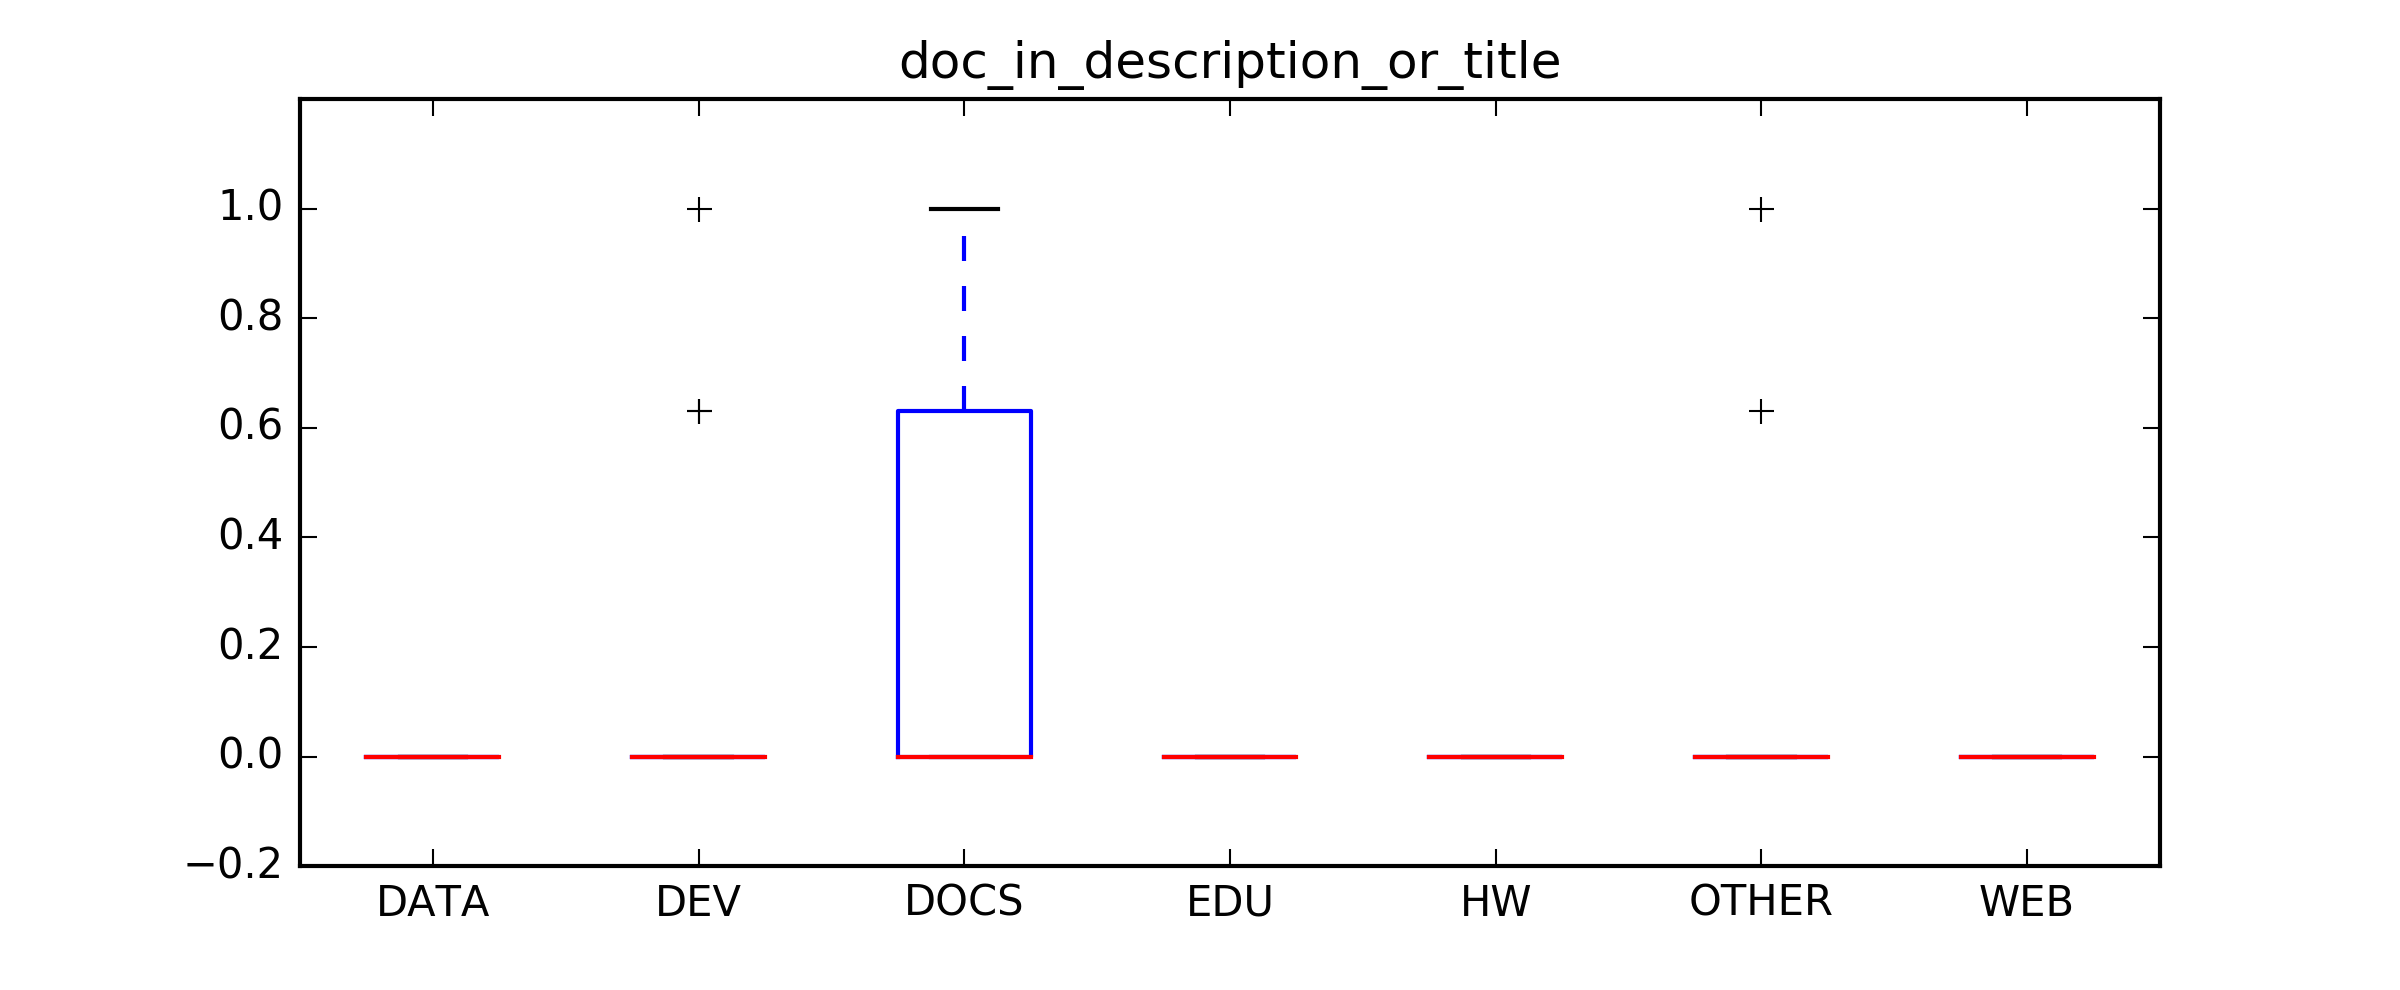
\includegraphics[width=0.75\linewidth]{figures/doc_in_description_or_title.png}
				\end{figure}
			\item[Forks count]
				This metric contains the number of forks for a repository.
				\begin{figure}[h!]
					\centering
					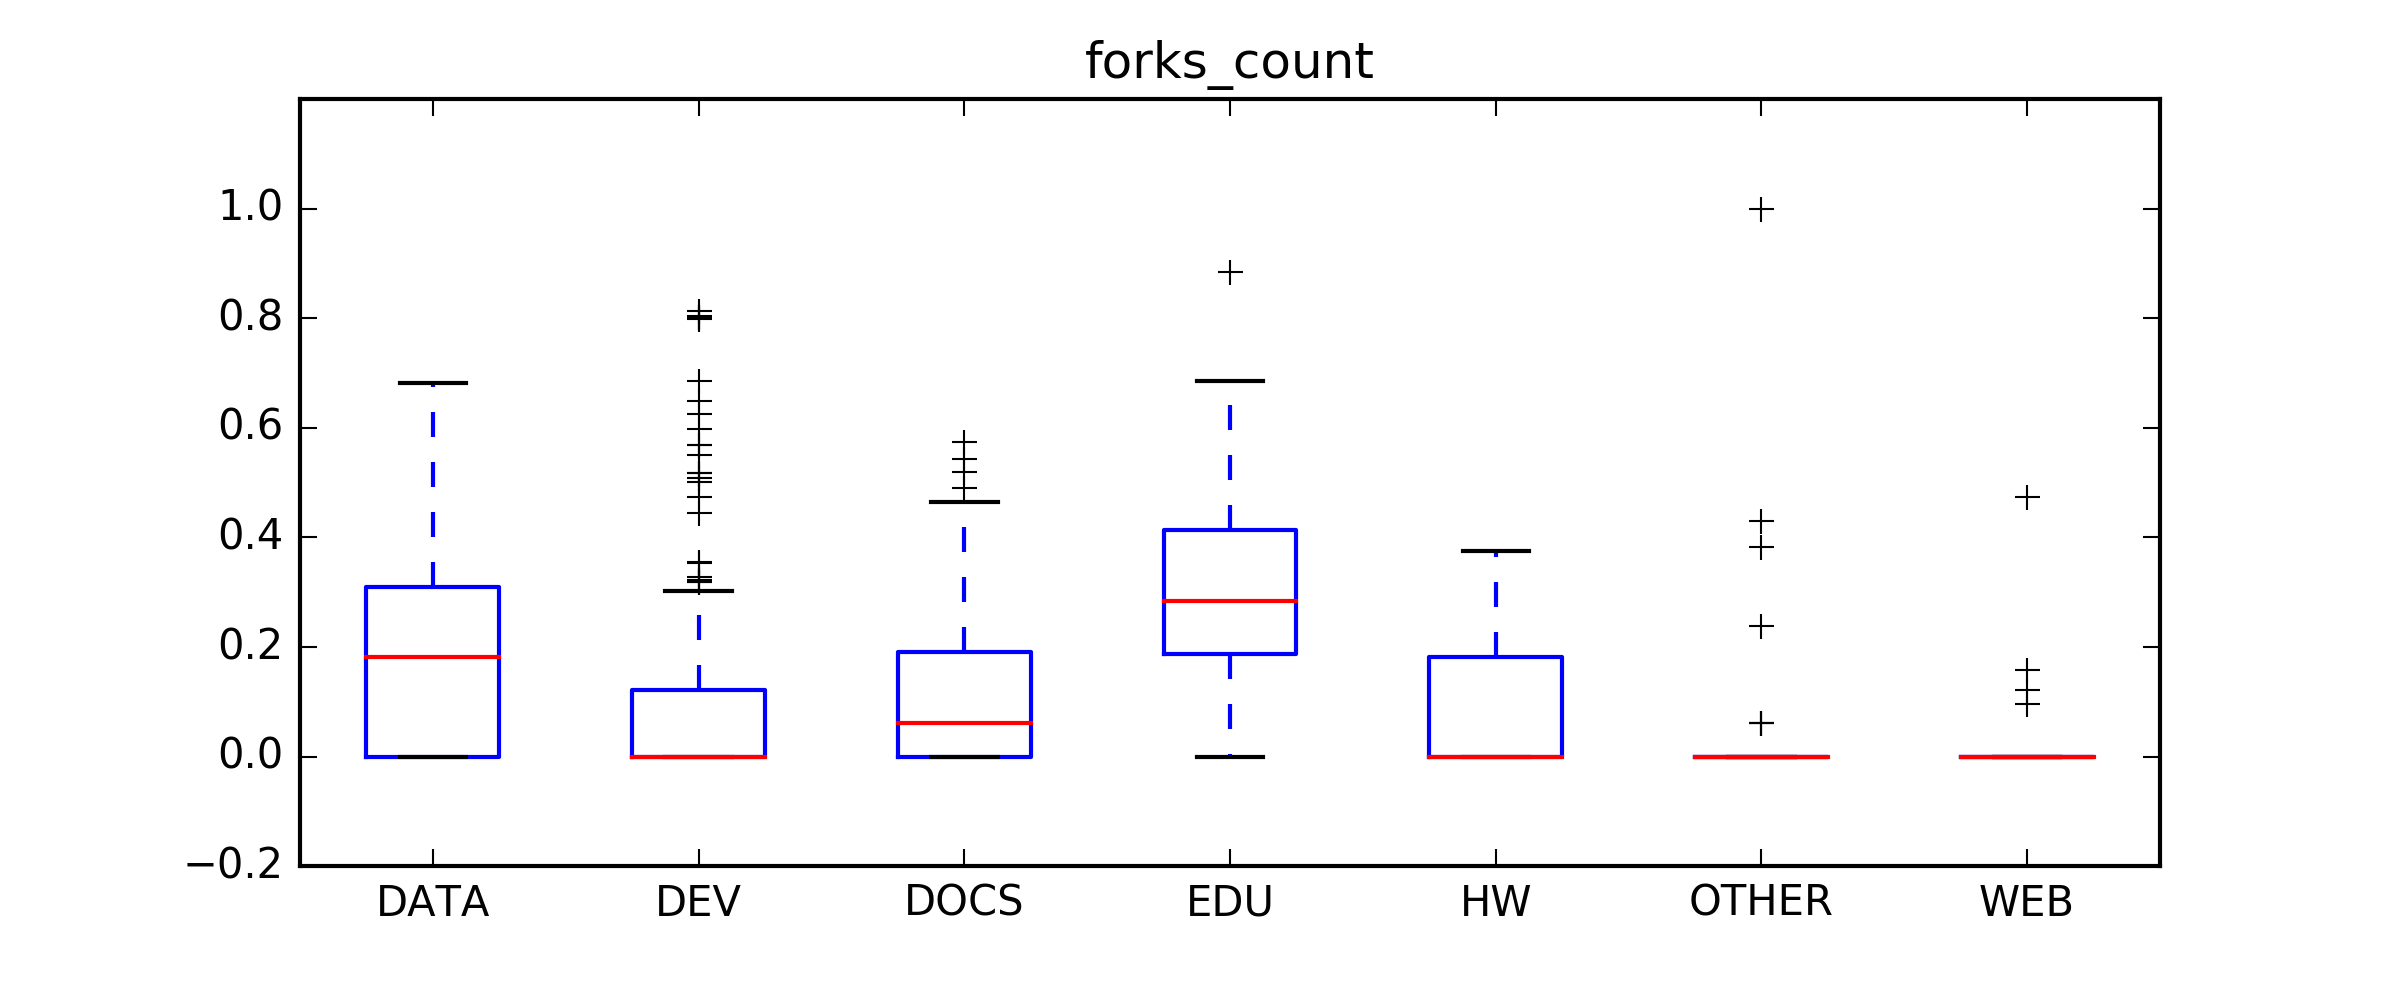
\includegraphics[width=0.75\linewidth]{figures/forks_count.png}
				\end{figure}
			\item[Homework terms in description or title]
				The terms 'homework' and 'assignment' in the repo description or title are strong indicators for a \emph{HW} repo.
				\begin{figure}[h!]
					\centering
					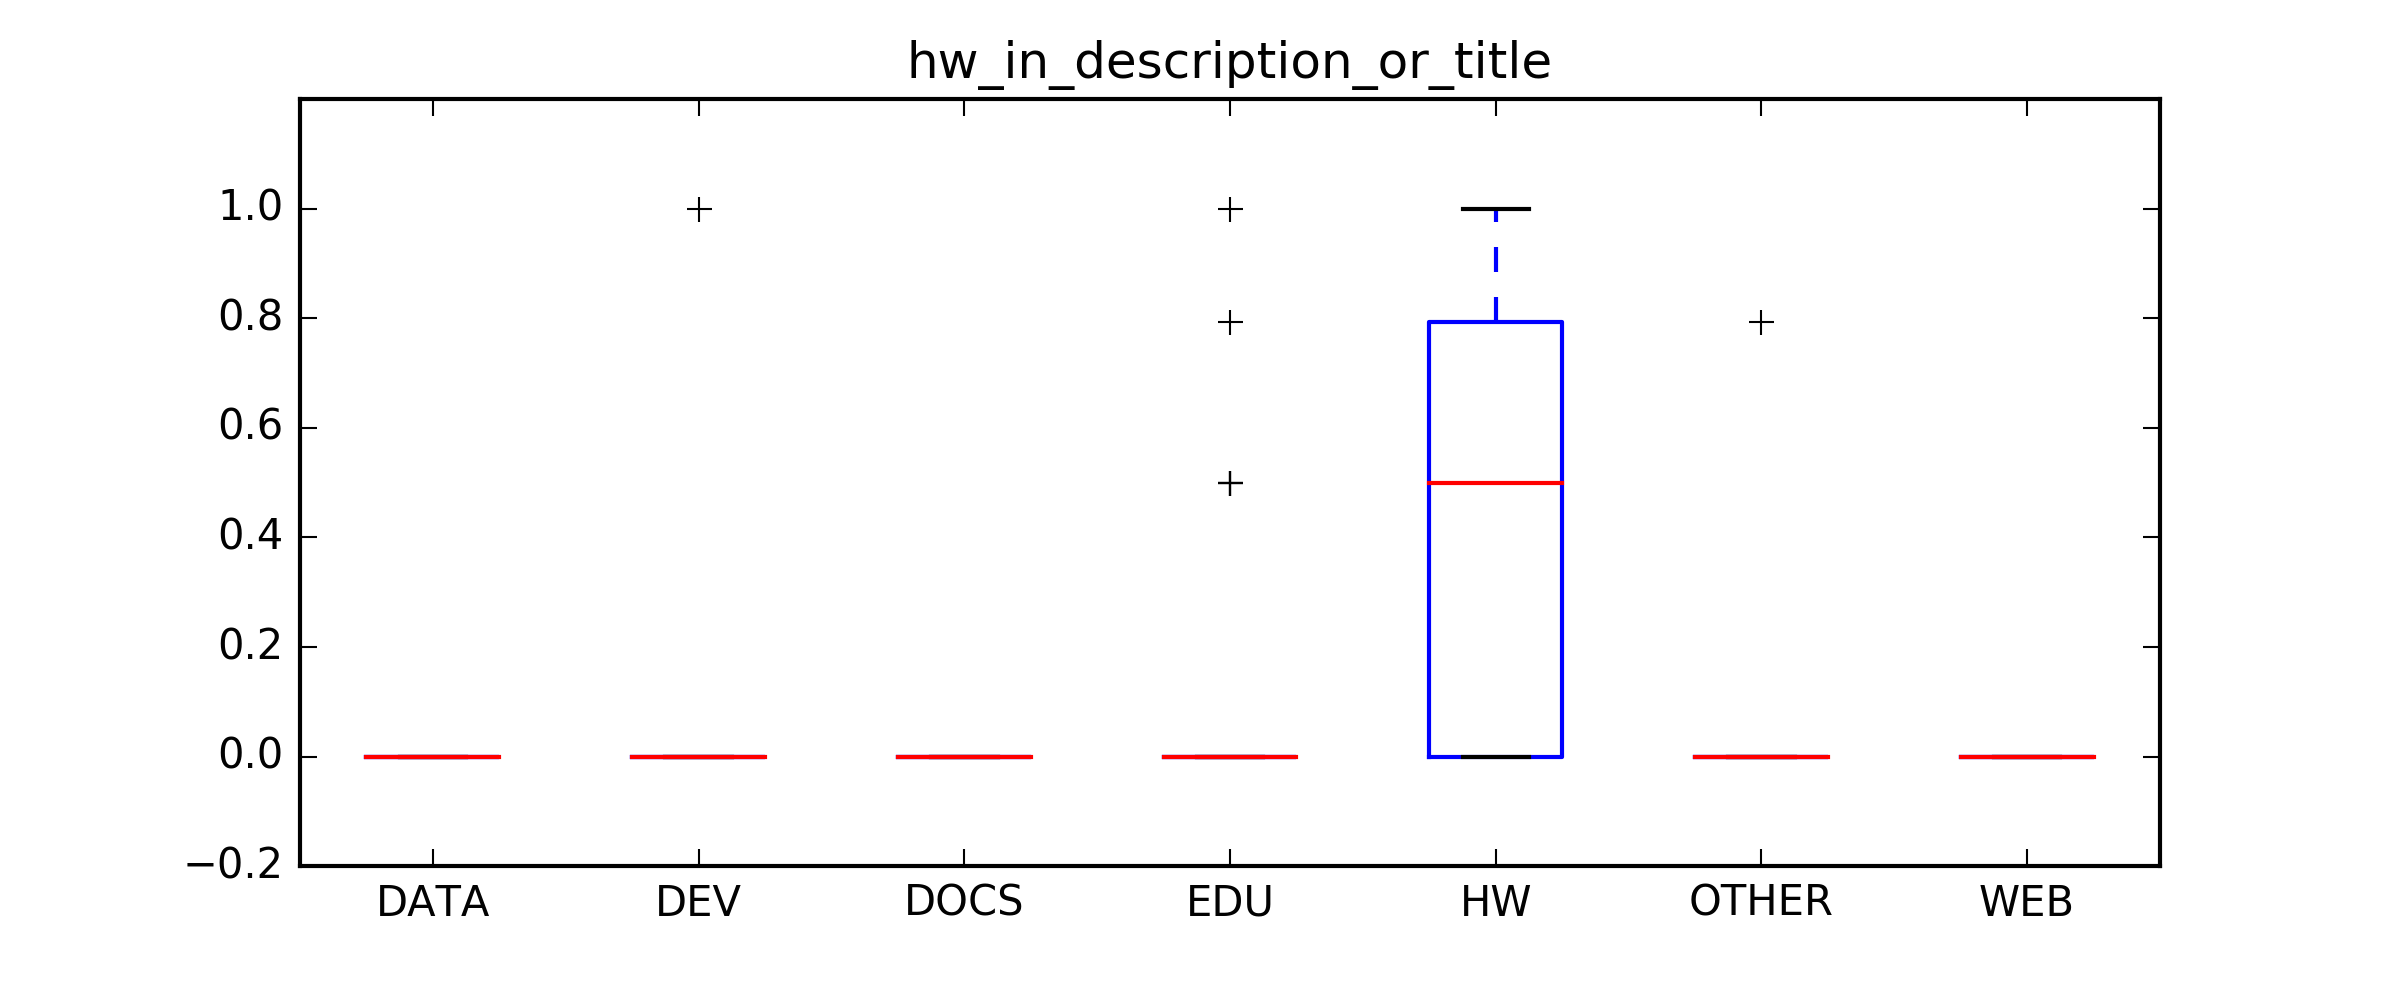
\includegraphics[width=0.75\linewidth]{figures/hw_in_description_or_title.png}
				\end{figure}
			\item[Intro or course in title or description]
				This metric searches for the terms 'intro' and 'course' in the repository title and description. If that is the case that is a strong indicator for a \emph{EDU} repository.
				\begin{figure}[h!]
					\centering
					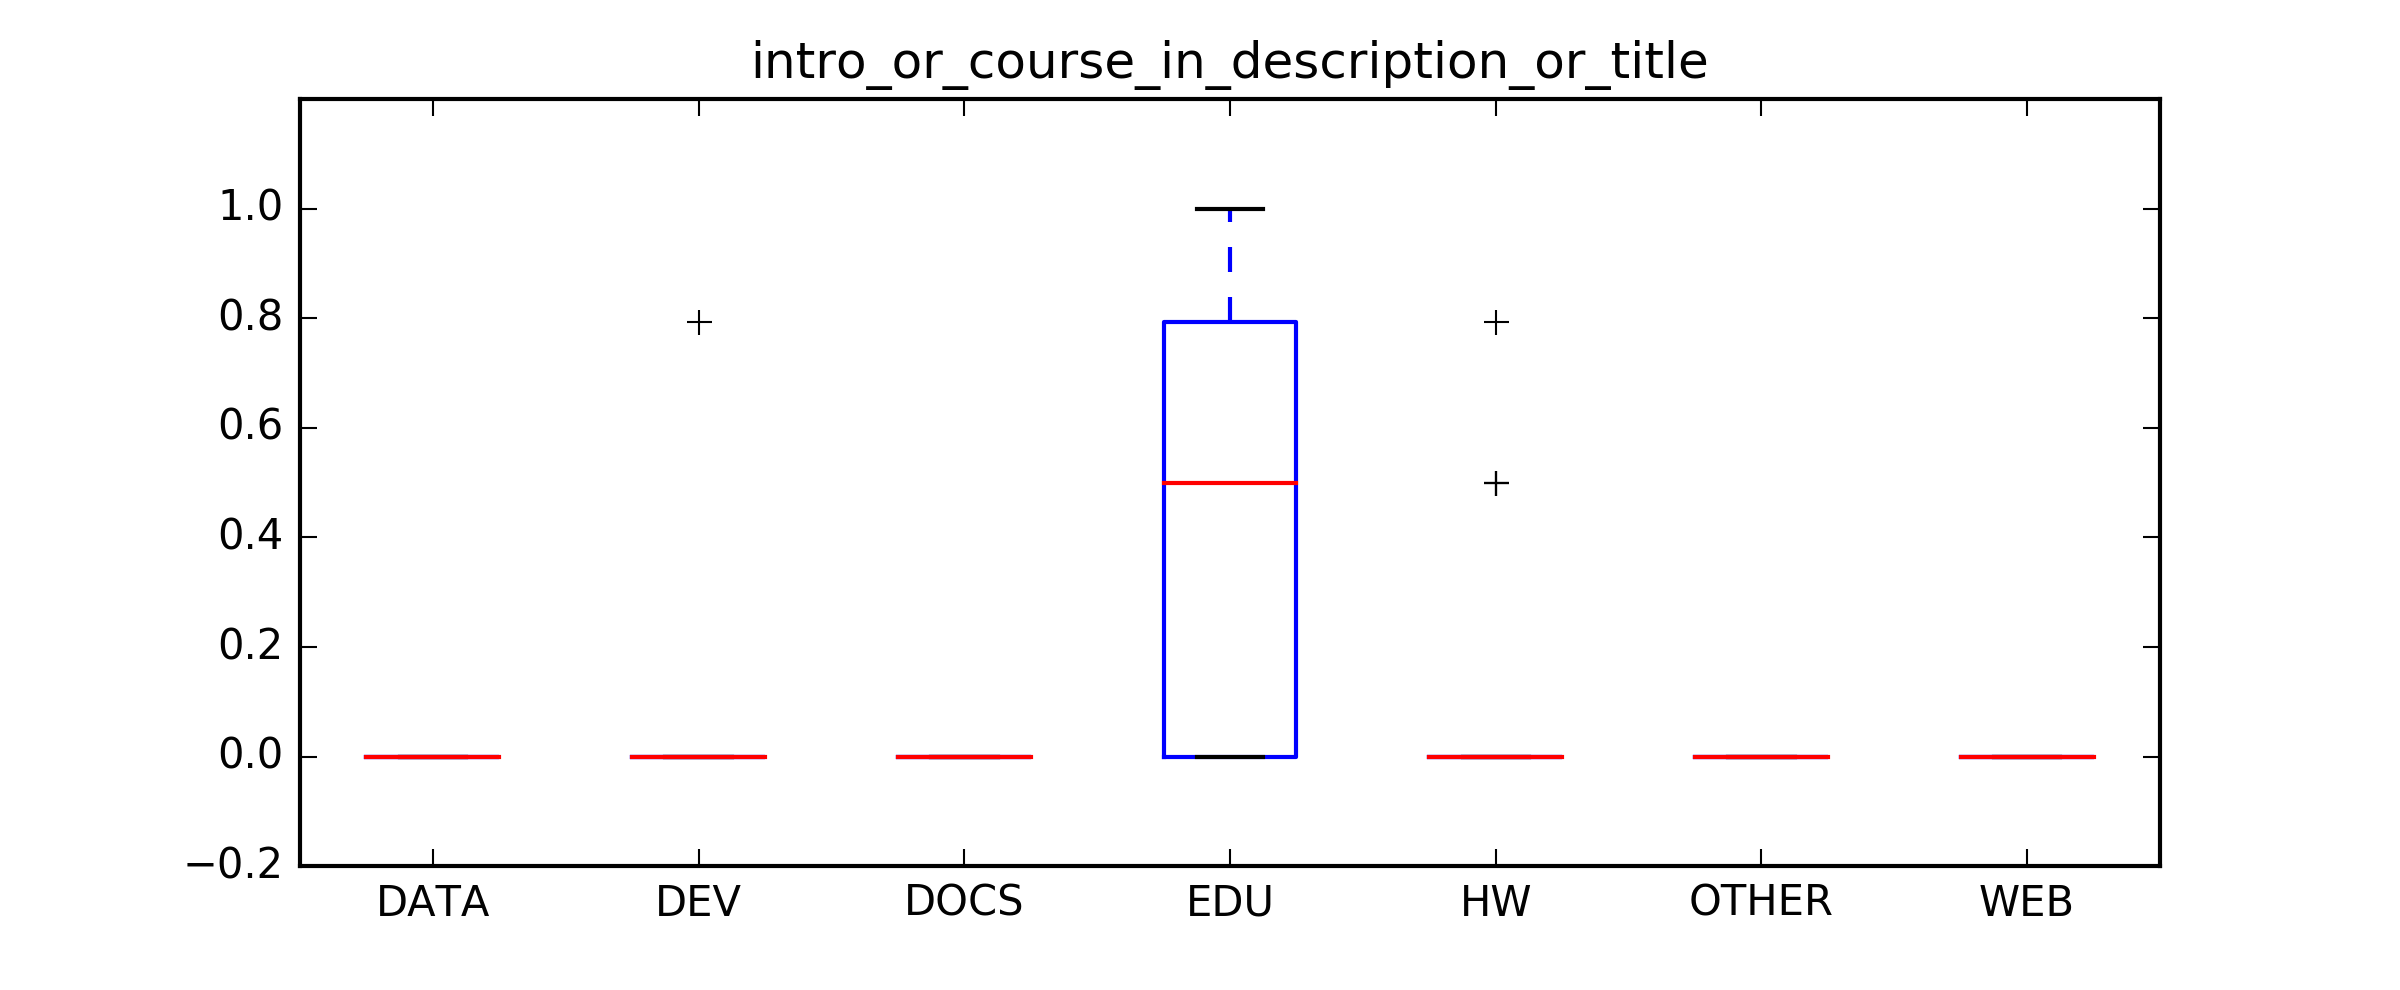
\includegraphics[width=0.75\linewidth]{figures/intro_or_course_in_description_or_title.png}
				\end{figure}
			\item[Is github.io page]
				Github host websites via Github pages. There are dedicated repositories with the name scheme <username>.github.io. This metrics helps us to identify such repositories as \emph{WEB}.
				\begin{figure}[h!]
					\centering
					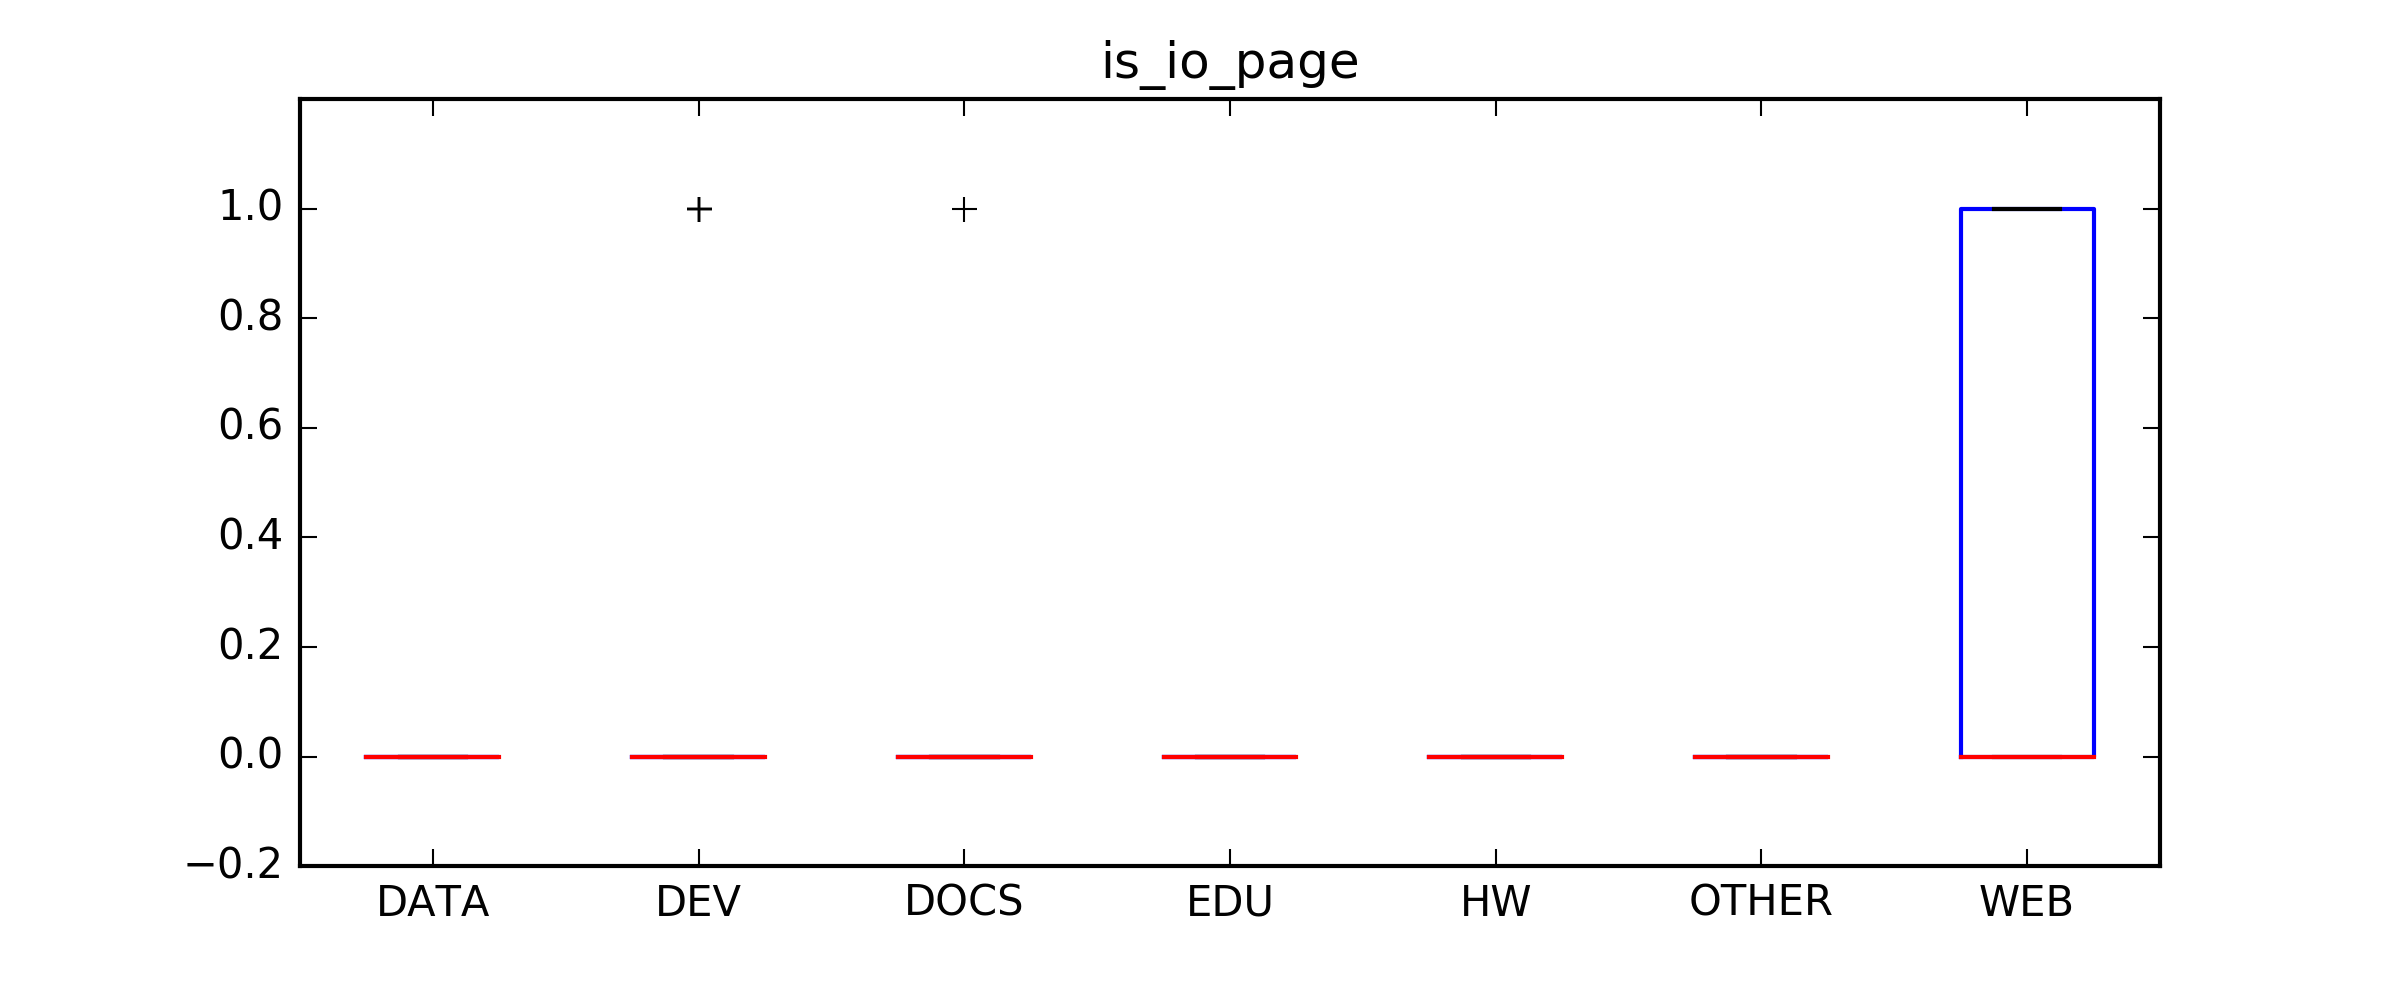
\includegraphics[width=0.75\linewidth]{figures/is_io_page.png}
				\end{figure}
			\item[Link in description]
				When looking at false predicted \emph{DOCS} repositories, we discovered, that they had links in the description, so we added this as a feature.
				\begin{figure}[h!]
					\centering
					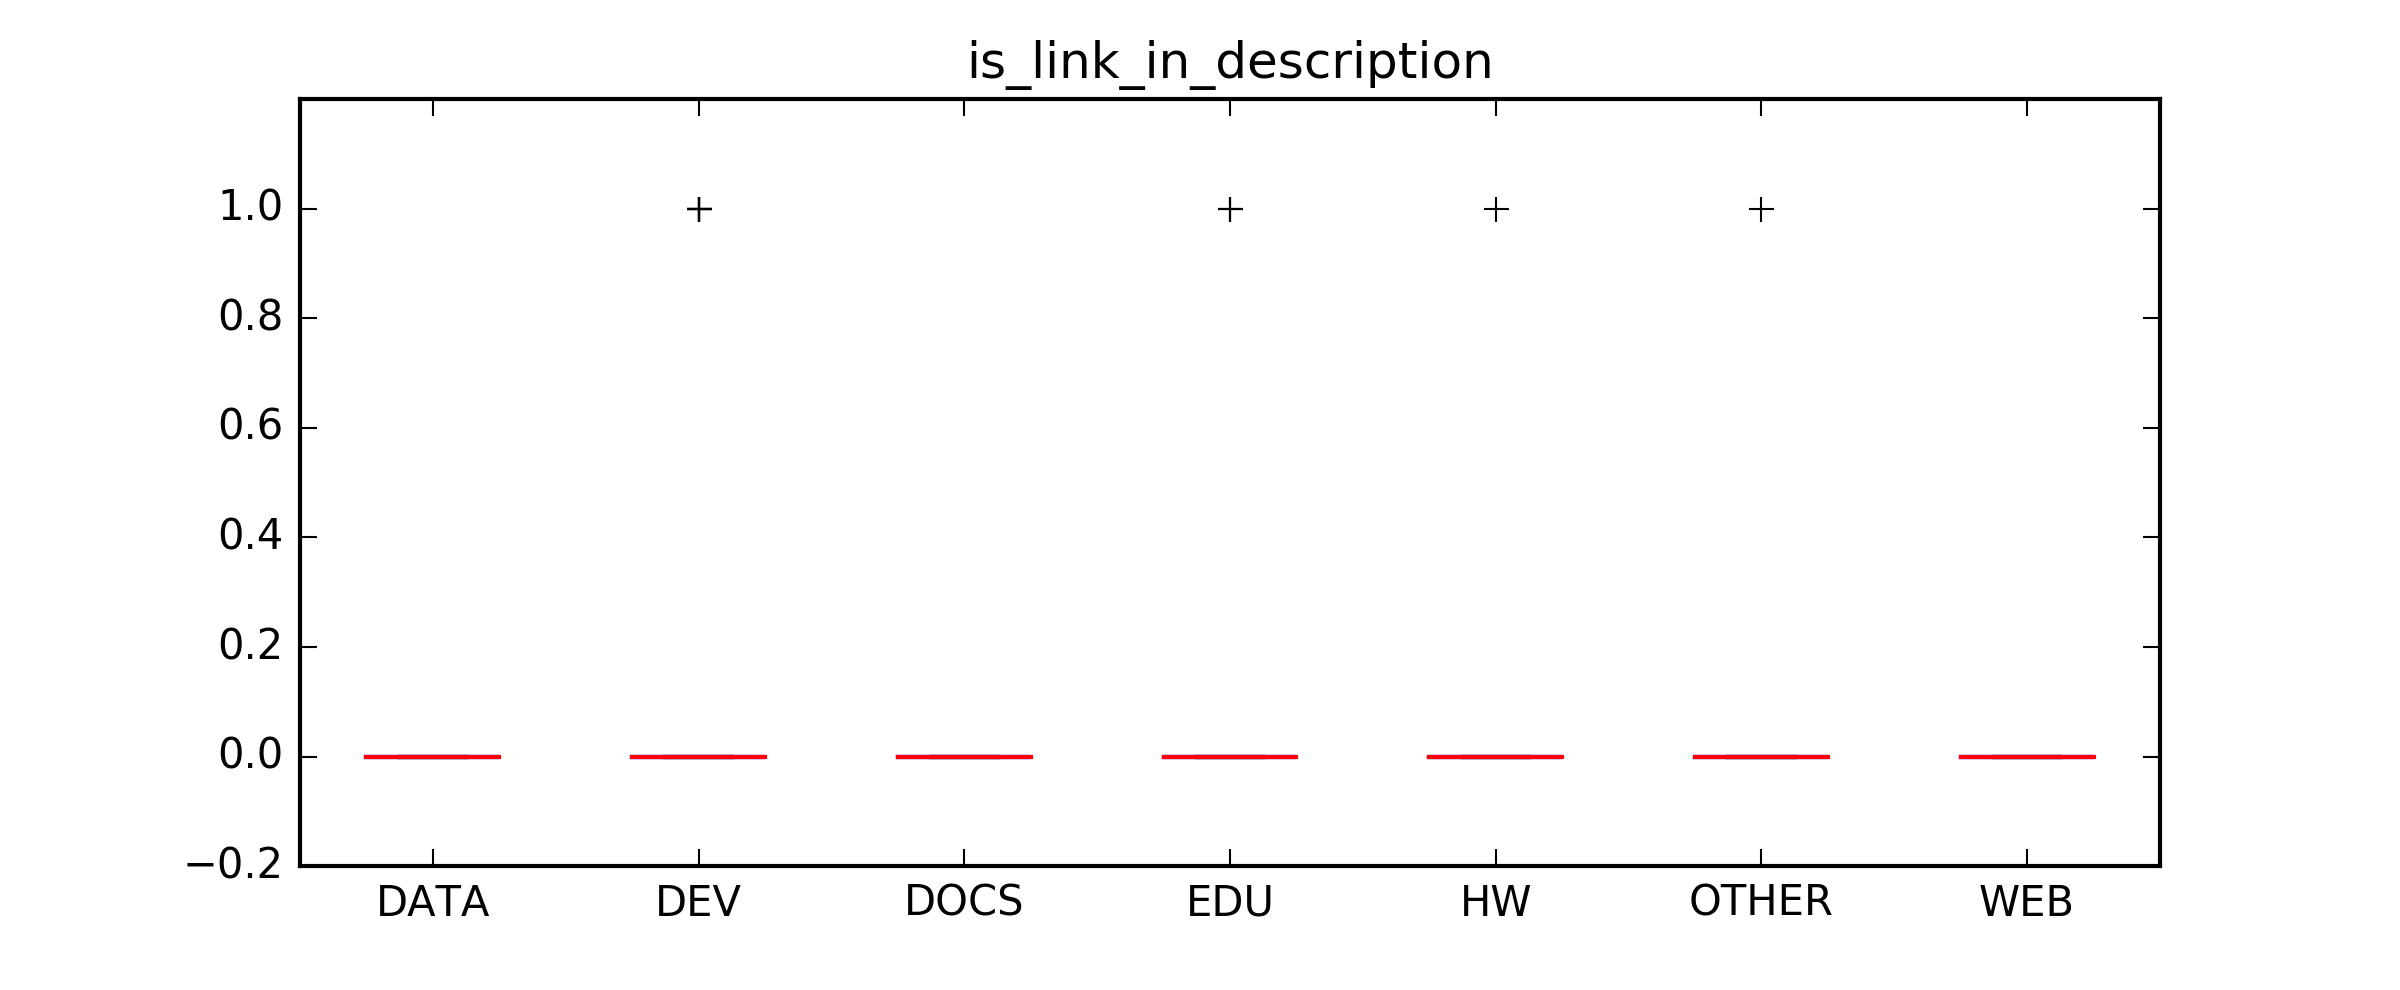
\includegraphics[width=0.75\linewidth]{figures/is_link_in_description.png}
				\end{figure}
			\item[Open issue count]
				The number of currently open issues. Many open issues indicate a popular repository. We expect mostly DEV to have a high open issue count.
				\begin{figure}[h!]
					\centering
					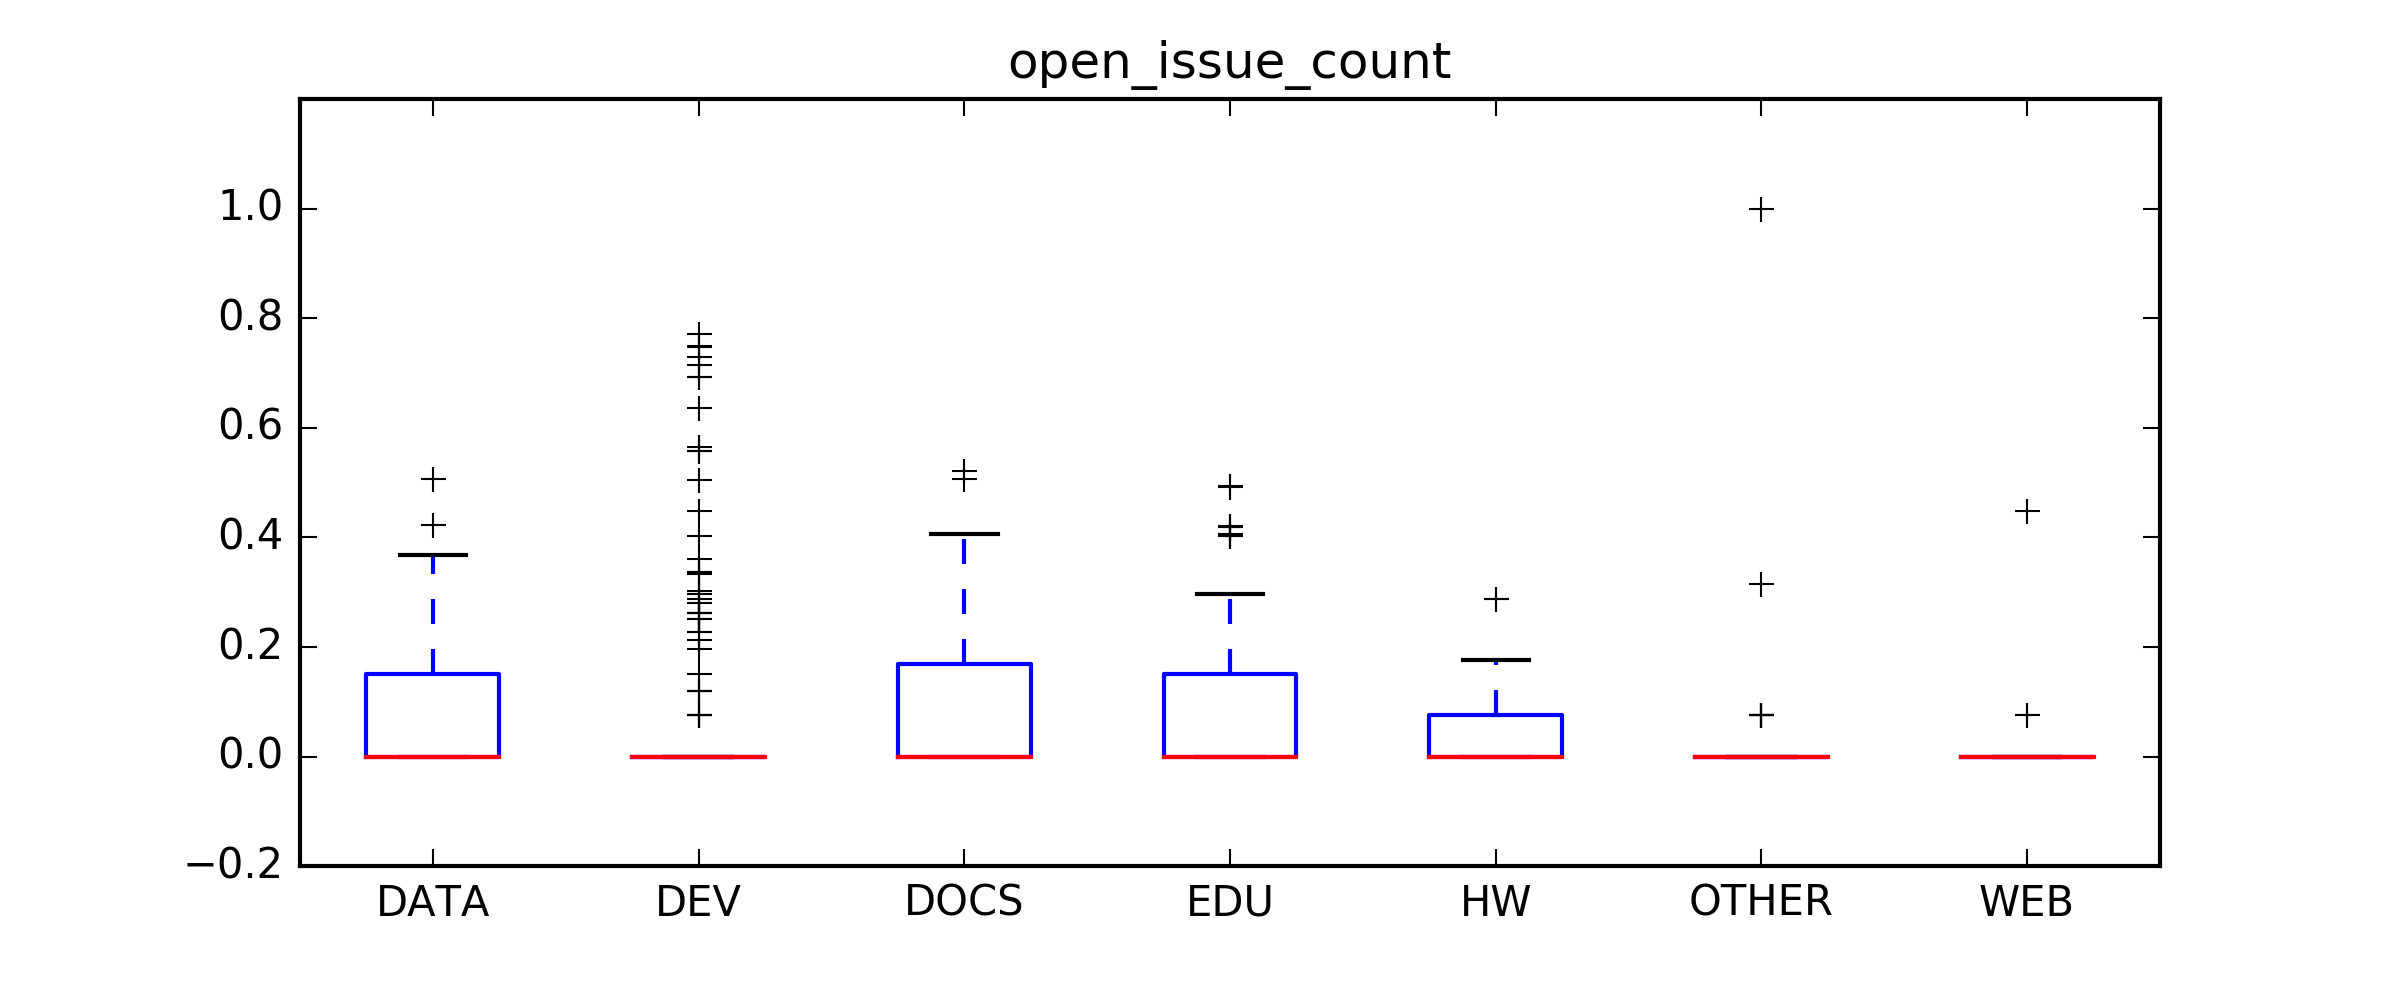
\includegraphics[width=0.75\linewidth]{figures/open_issue_count.png}
				\end{figure}
			\item[Repository size]
				The repository size in kilobytes. Repositories of each category can have a small size but we only expect \emph{DEV}, \emph{DOCS}, \emph{DATA} and \emph{WEB} repository to have a big size.
				\begin{figure}[h!]
					\centering
					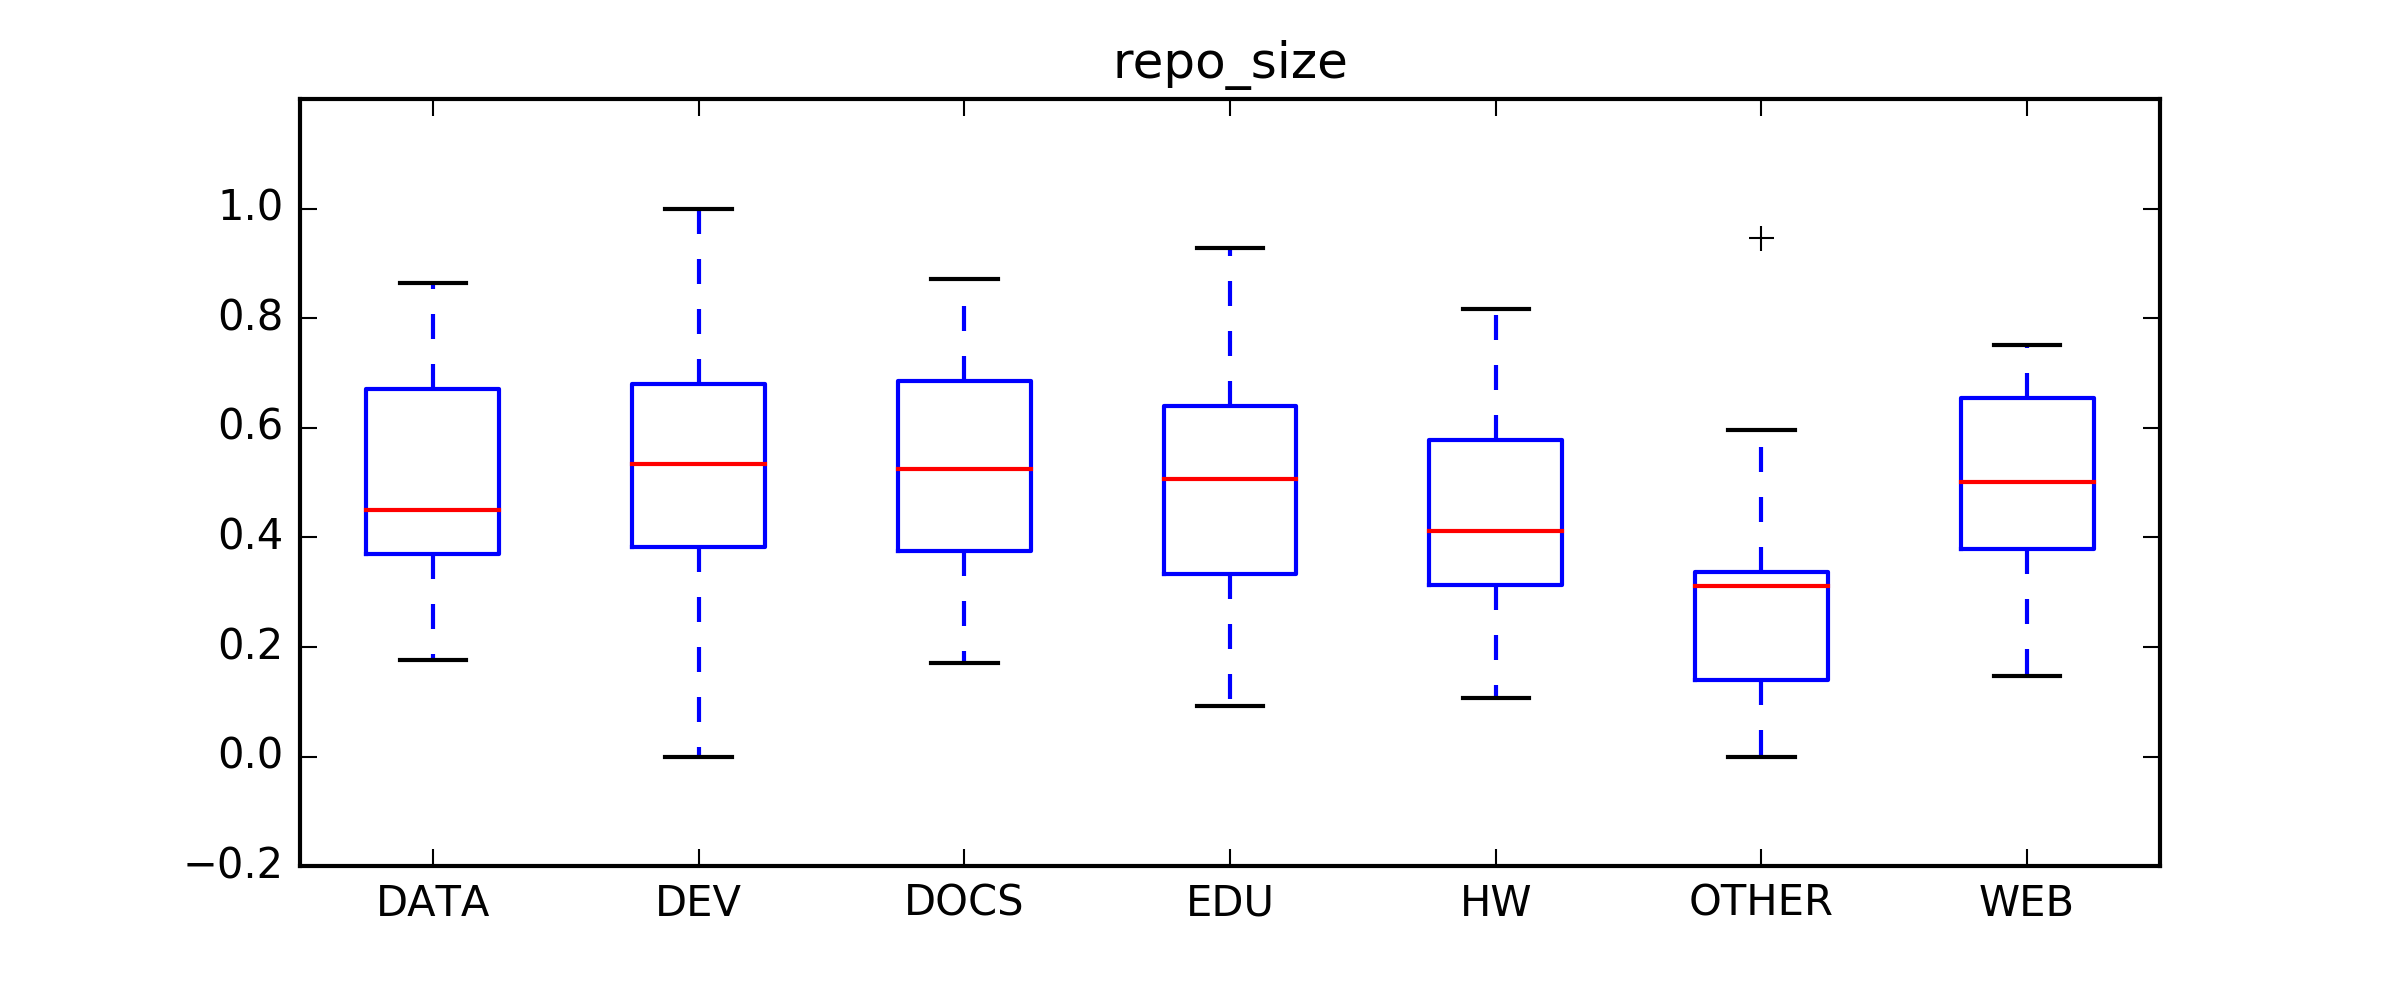
\includegraphics[width=0.75\linewidth]{figures/repo_size.png}
				\end{figure}
			\item[Up-to-dateness]
				Measures the time since the last commit. We expect HW repositories to have a low up-to-dateness because they are not worked on after deadline.
				\begin{figure}[h!]
					\centering
					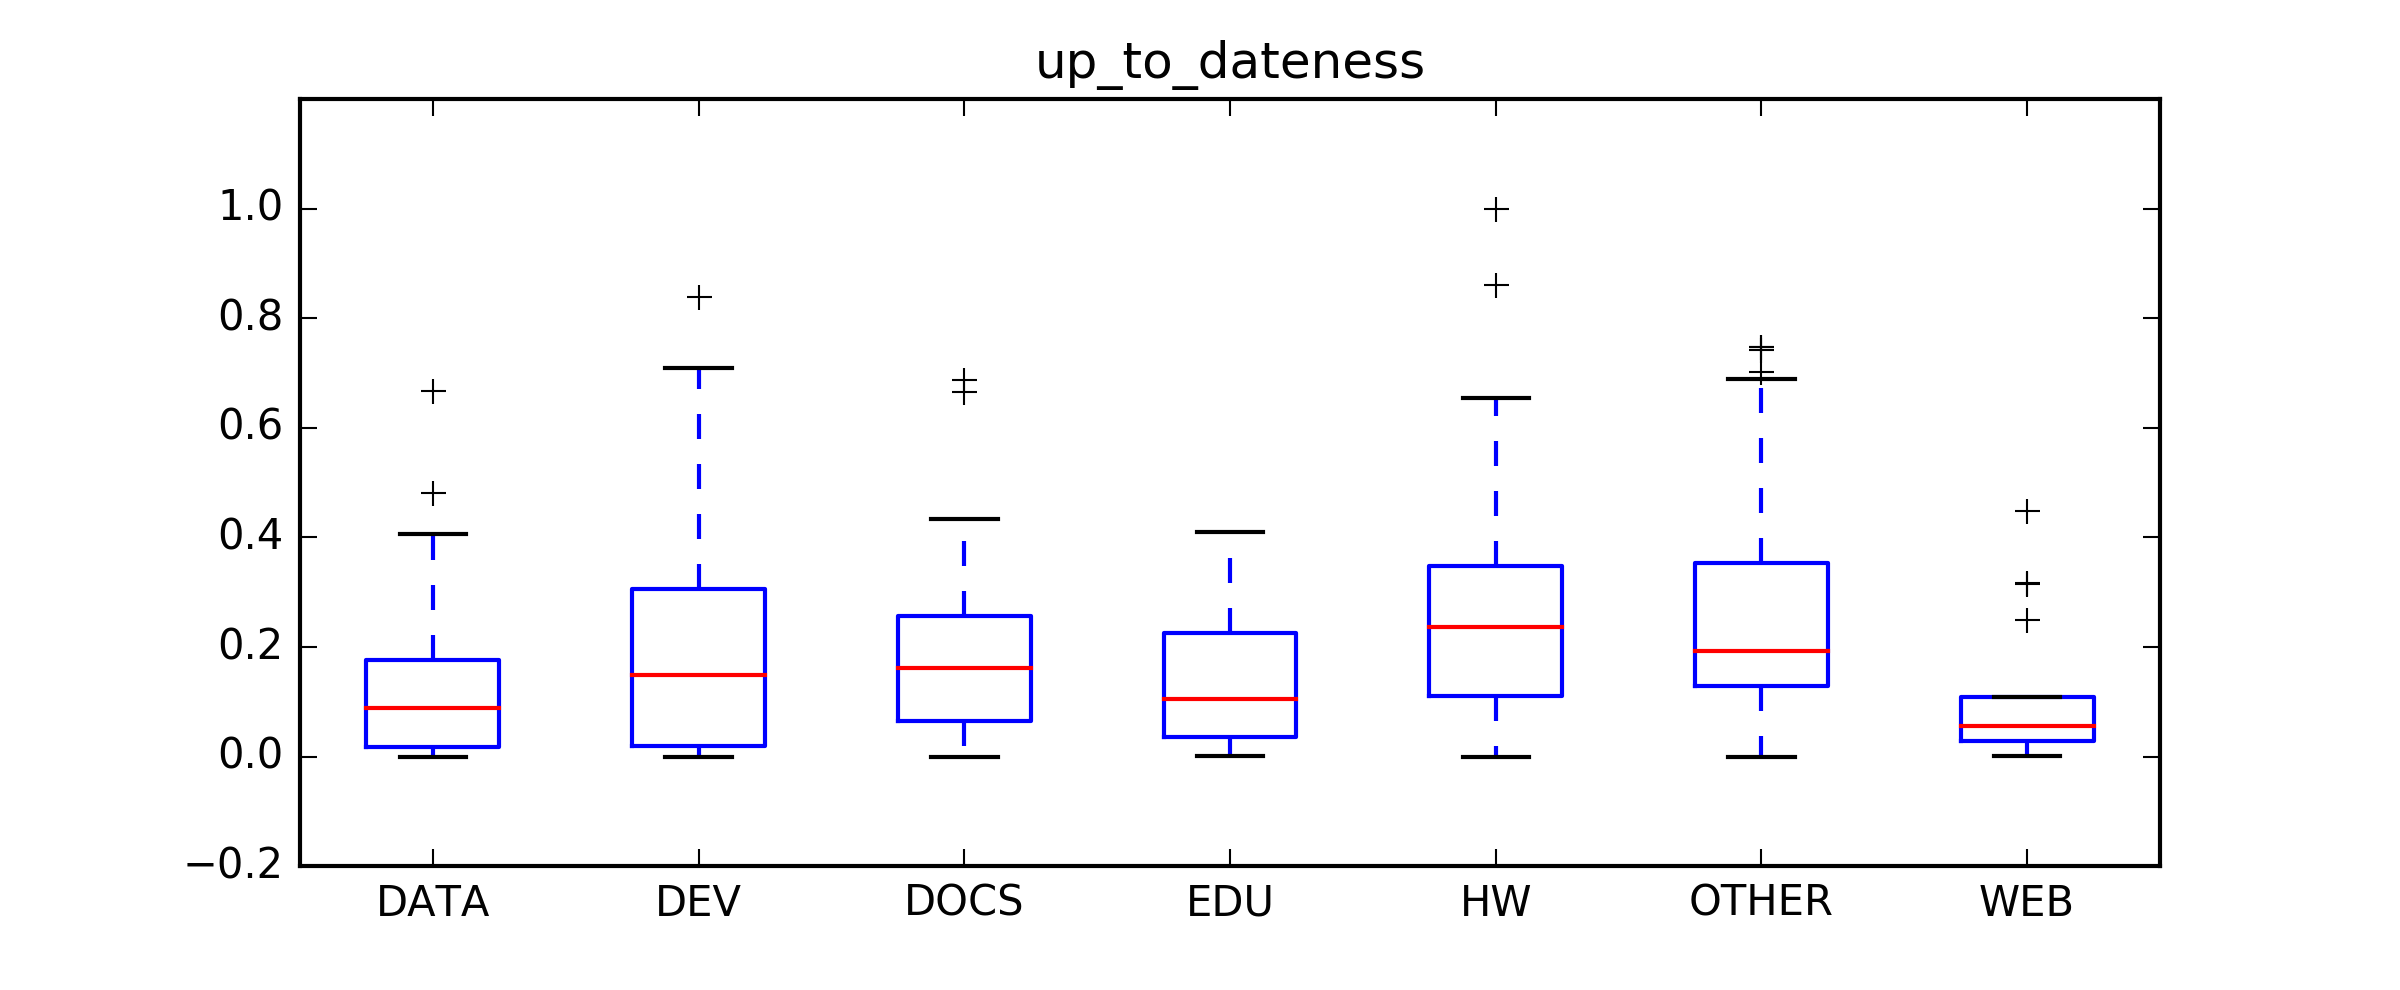
\includegraphics[width=0.75\linewidth]{figures/up_to_dateness.png}
				\end{figure}
			\item[Watcher count]
				The watcher count indicates the popularity of a repository. We expect only \emph{DEV} repositories to have a high watcher count. \emph{EDU} could also have an higher than average watcher count.
				\begin{figure}[h!]
					\centering
					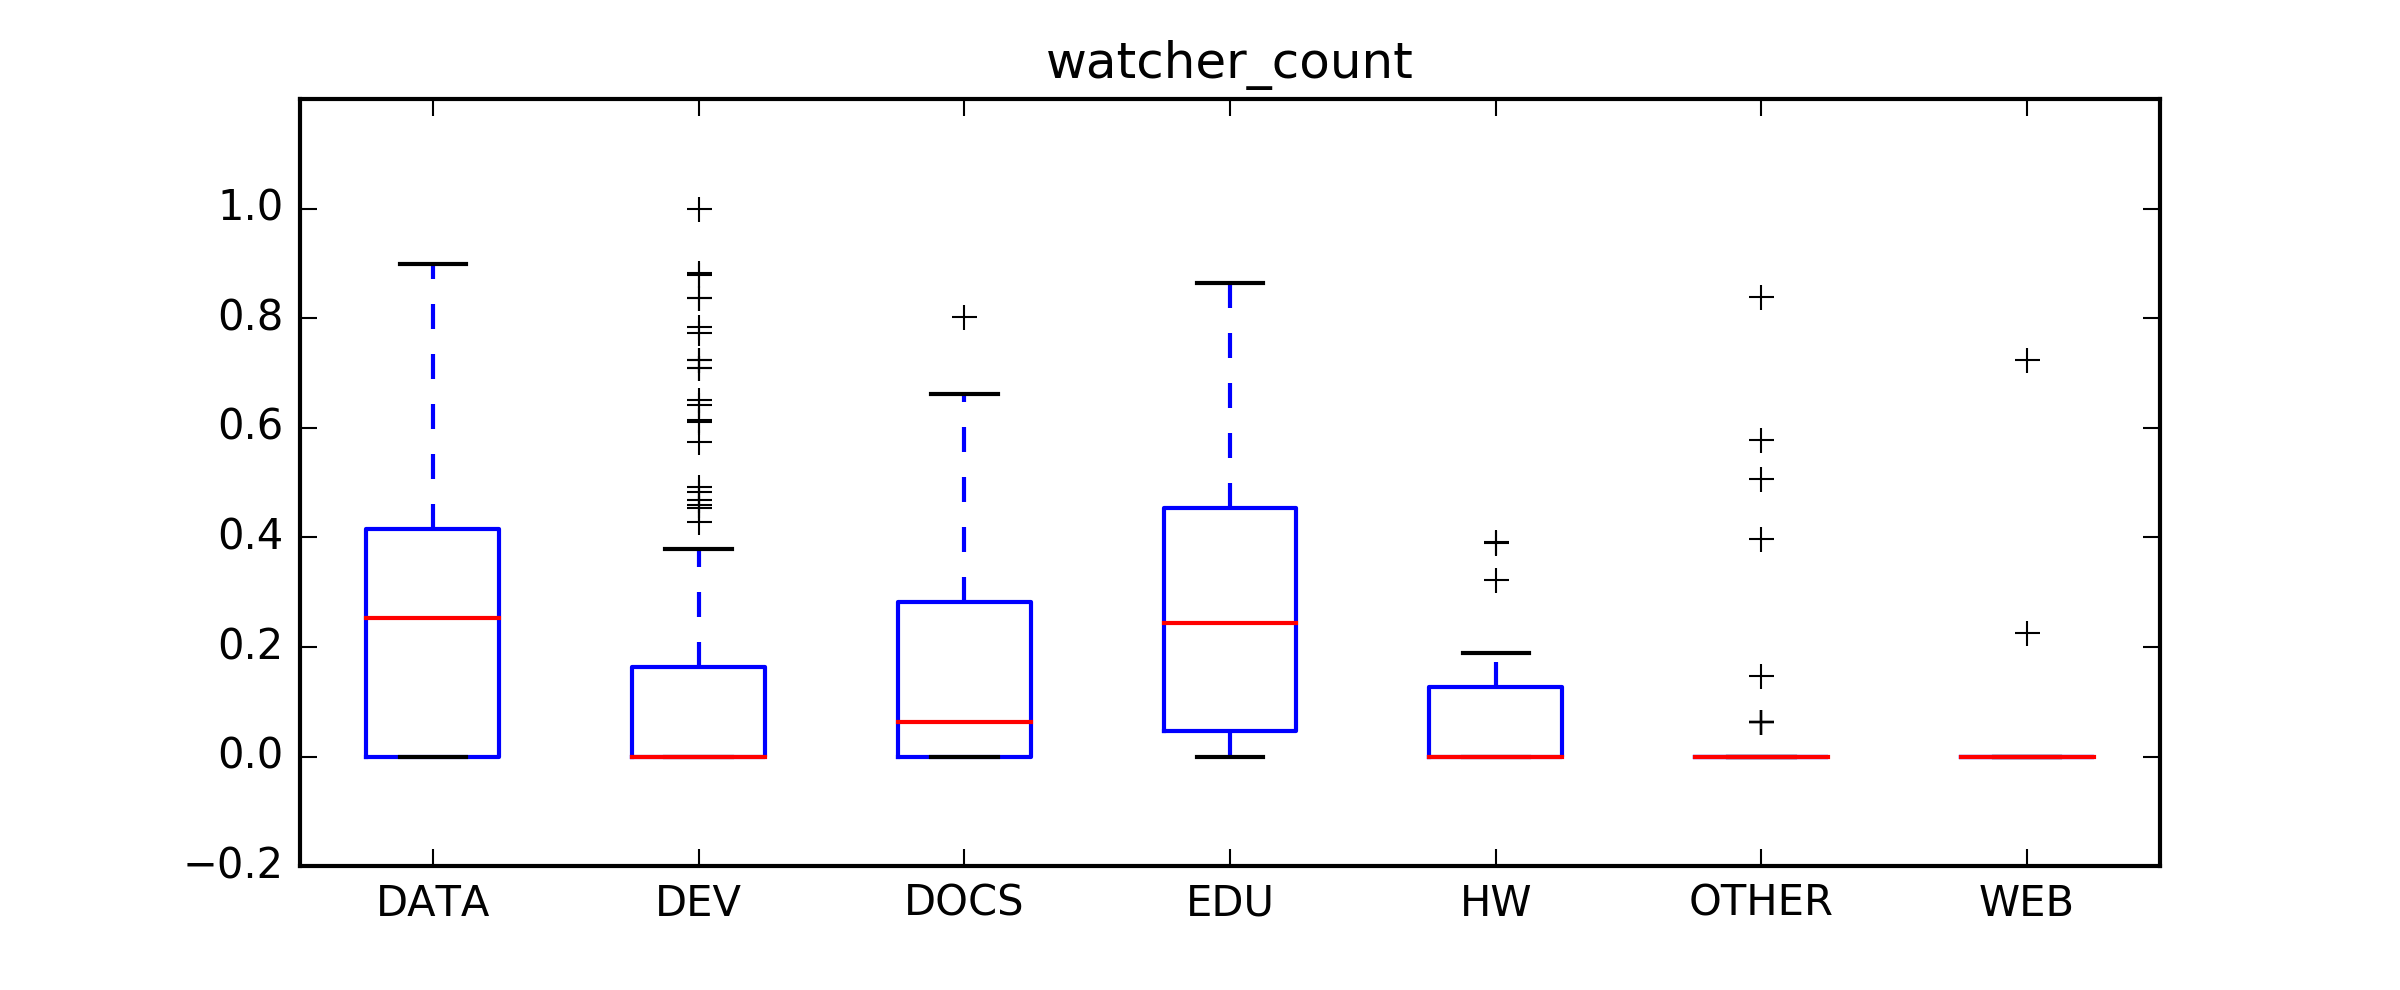
\includegraphics[width=0.75\linewidth]{figures/watcher_count.png}
				\end{figure}
		\end{description}
		
		% subsubsection api_repo_overview (end)

		\subsubsection{cloned repository} % (fold)
		\label{ssub:cloned_repository}

		% 'avg_entropy',
		% 'avg_folder_depth',
		% 'doc_terms_in_readme',
		% 'edu_mail_ratio'
		% 'file_count',
		% 'file_folder_ratio',
		% 'html_count',
		% 'hw_terminology_commits',
		% 'hw_terminology_file_or_dir_names',
		% 'md_count',
		% 'pdf_count',
		% 'png_count',
		% 'source_code_file_ratio',
		
		\begin{description}
			\item[Average entropy]
				The entropy of each repository file is calculated and the average of all these files is returned. We expect \emph{DATA} and \emph{EDU} to have a high entropy because of many pictures and videos. \emph{DOCS} and \emph{WEB} have a medium entropy because of some pictures. \emph{DEV} and \emph{HW} have a low entropy because they contain mostly source code. Is actually helps to predict \emph{OTHER} really well, because of an entropy of 0.3 or lower.
				\begin{figure}[h!]
					\centering
					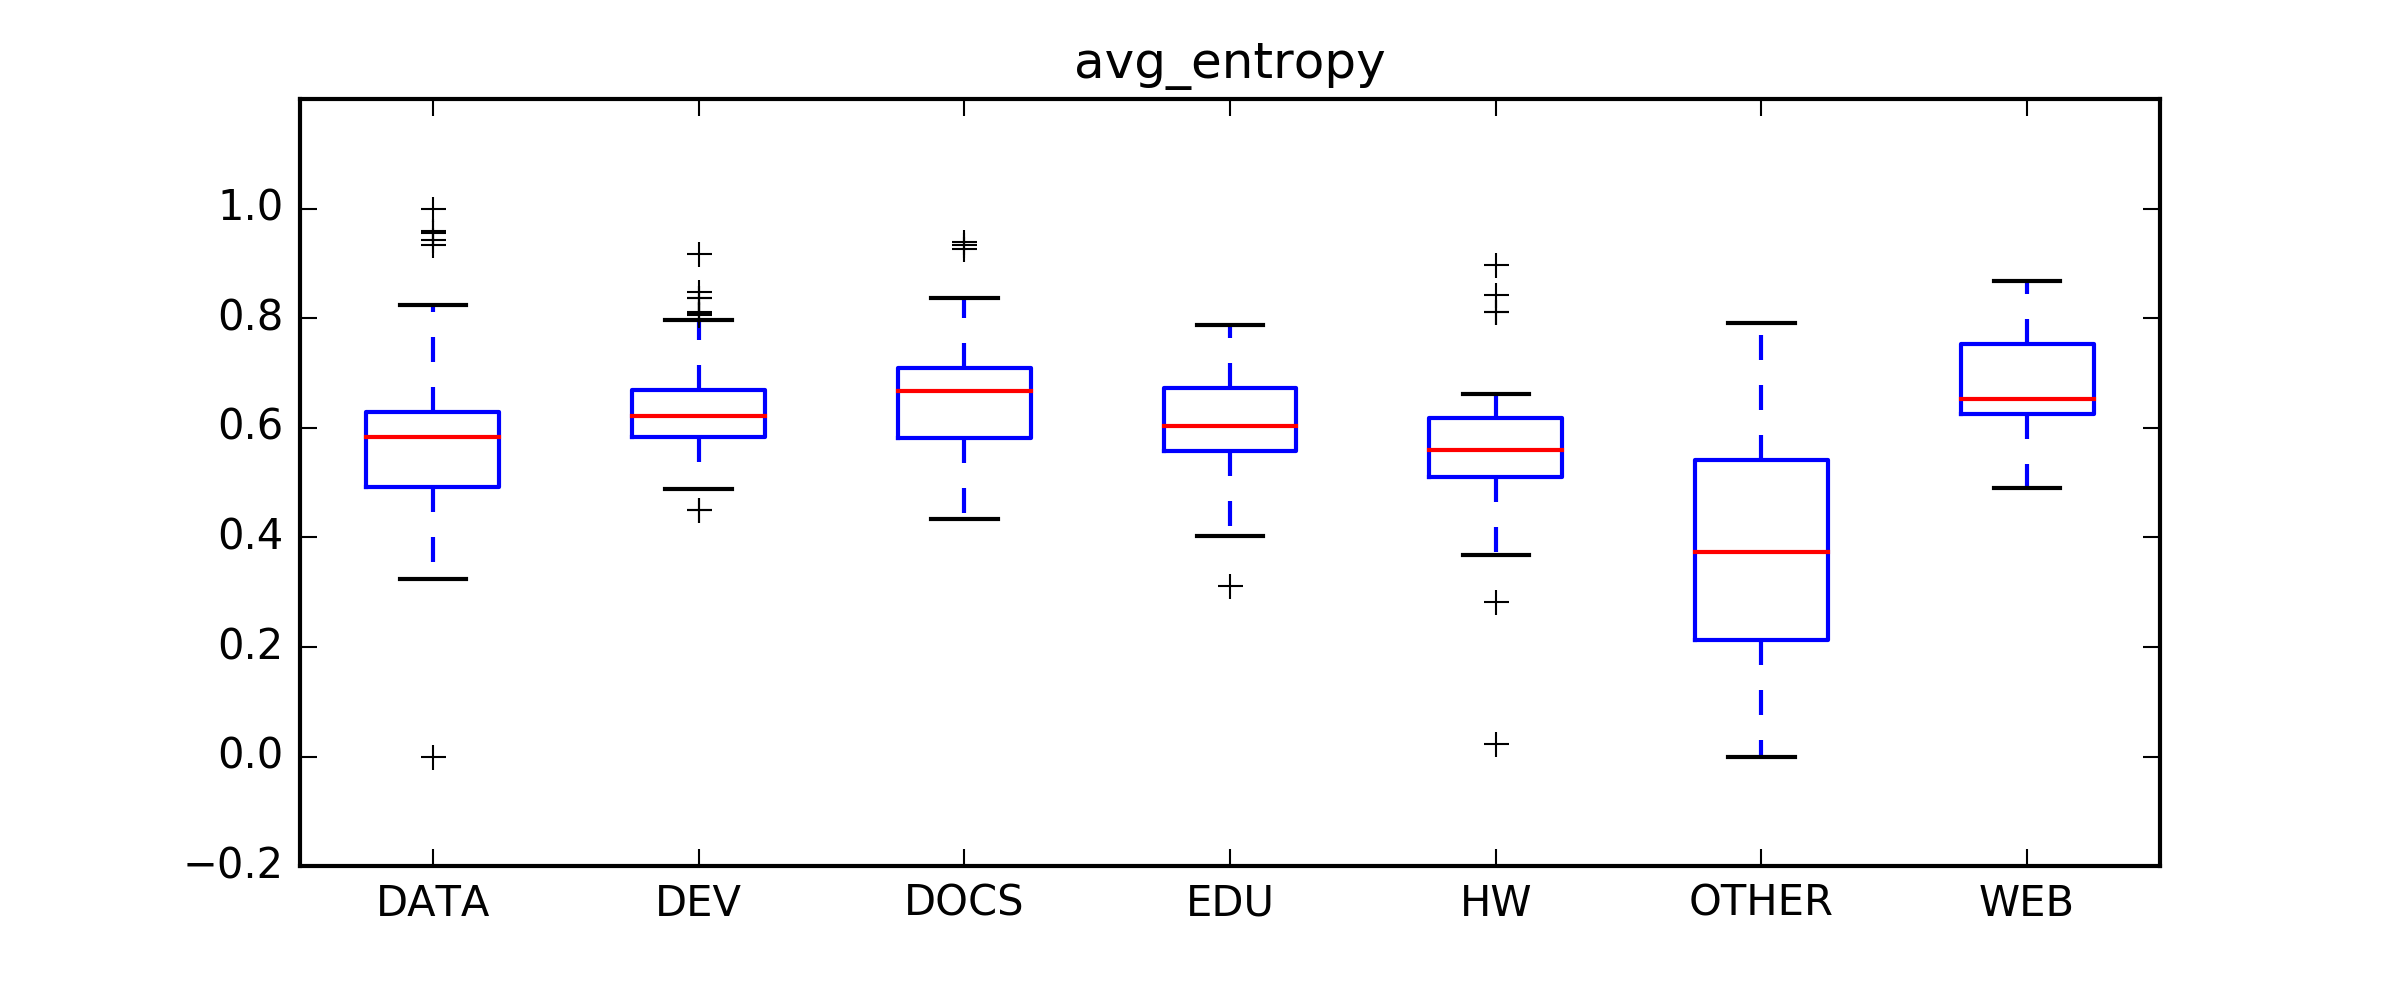
\includegraphics[width=0.75\linewidth]{figures/avg_entropy.png}
				\end{figure}
			\item[Average folder depth]
				This averages the depth of all folders. We expected Java repos to have a deep folder structure, but \emph{HW} to a flat one.
				\begin{figure}[h!]
					\centering
					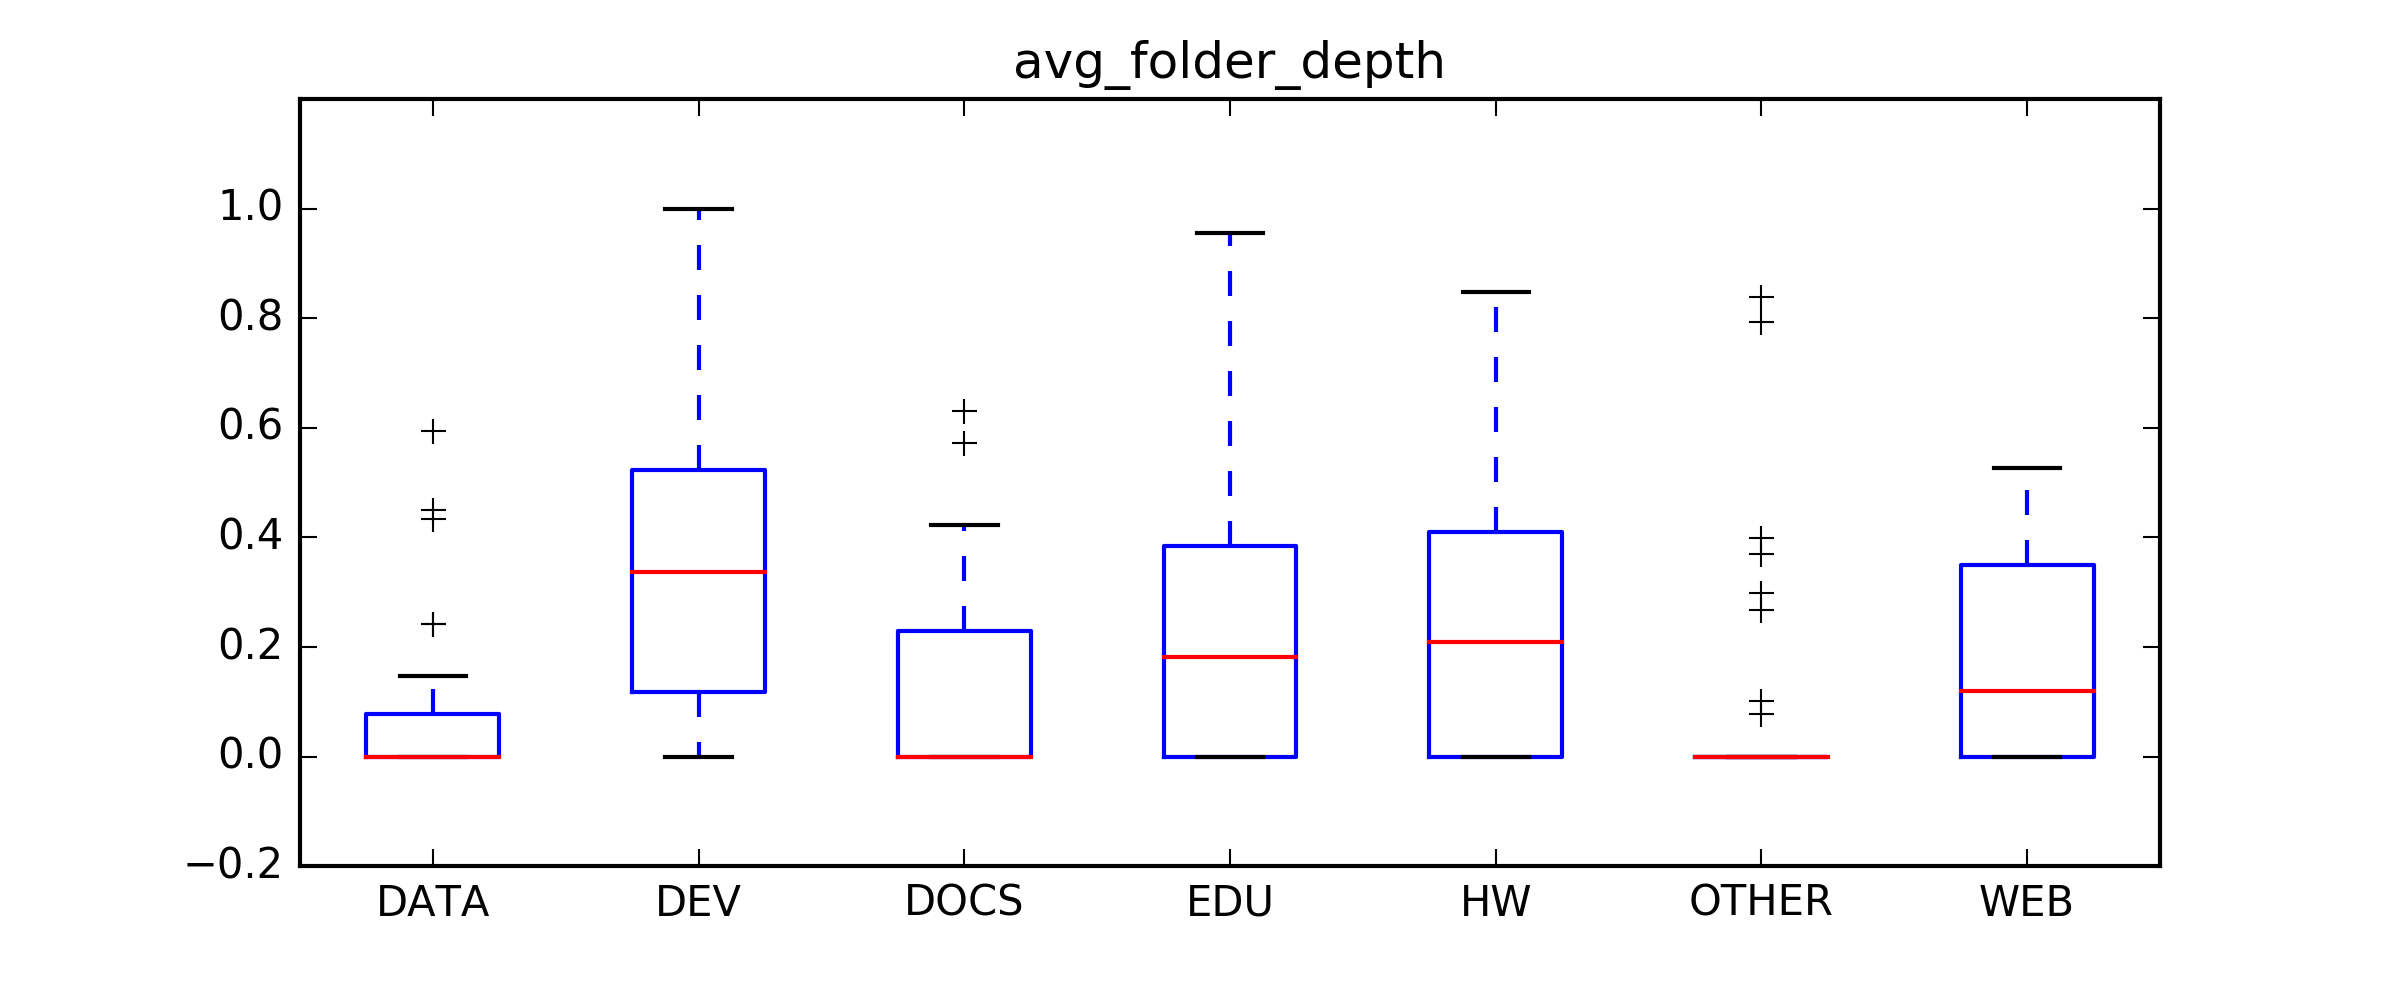
\includegraphics[width=0.75\linewidth]{figures/avg_folder_depth.png}
				\end{figure}
			\item[DOC terms in read me]
				Returns the number of common DOC terms in the Readme file. Under common DOC terms we understand: 'documentation', 'usage', 'guide', 'installation', 'getting started', 'quickstart', 'tutorial' and 'setup'.
				\begin{figure}[h!]
					\centering
					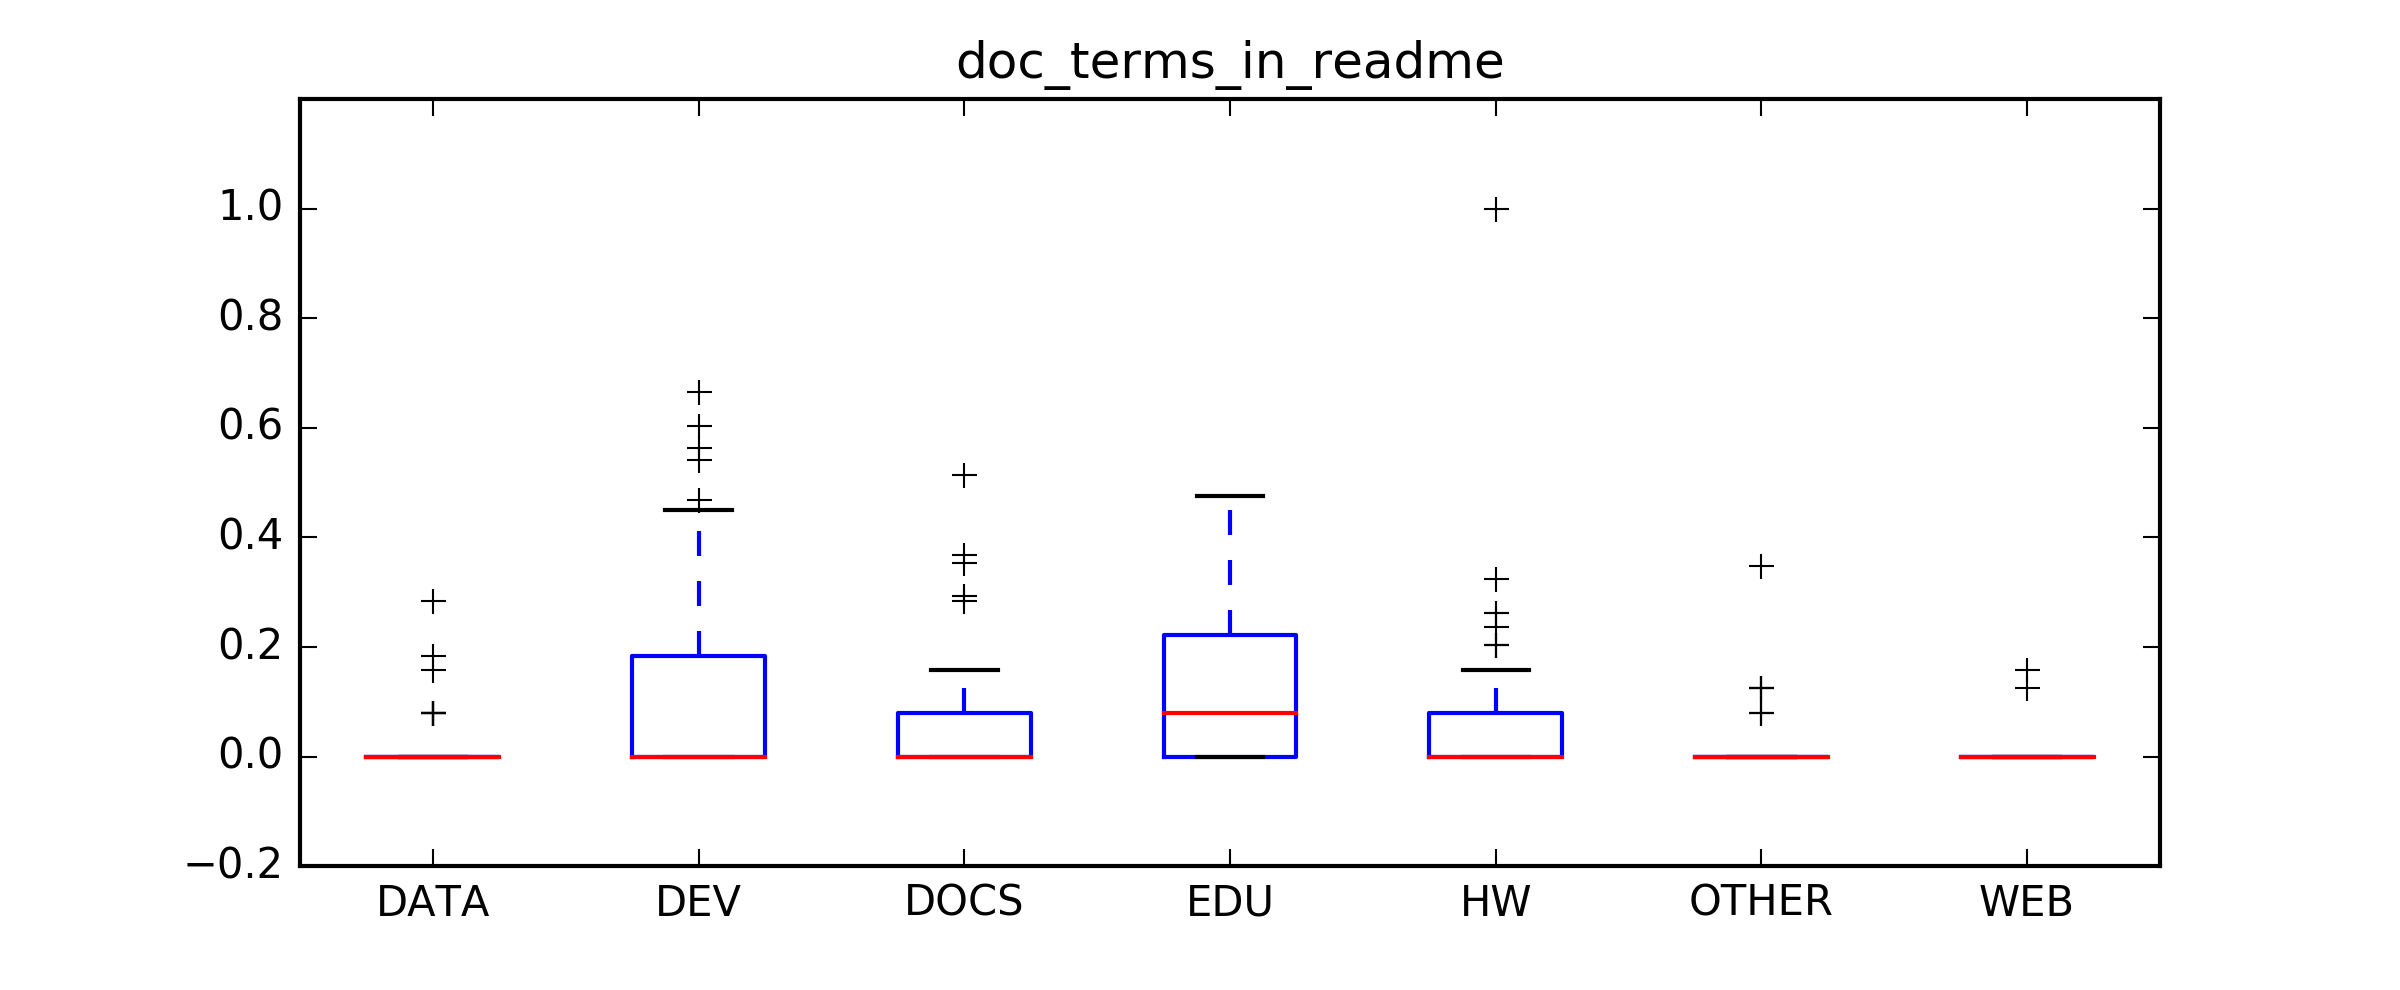
\includegraphics[width=0.75\linewidth]{figures/doc_terms_in_readme.png}
				\end{figure}
			\item[Education e-mail ratio]
				This is the ration between university mail addresses to all unique addresses that appear in a repository. We extract them from the commit messages. We expect \emph{EDU} to have a high \emph{EDU} mail ratio.
				\begin{figure}[h!]
					\centering
					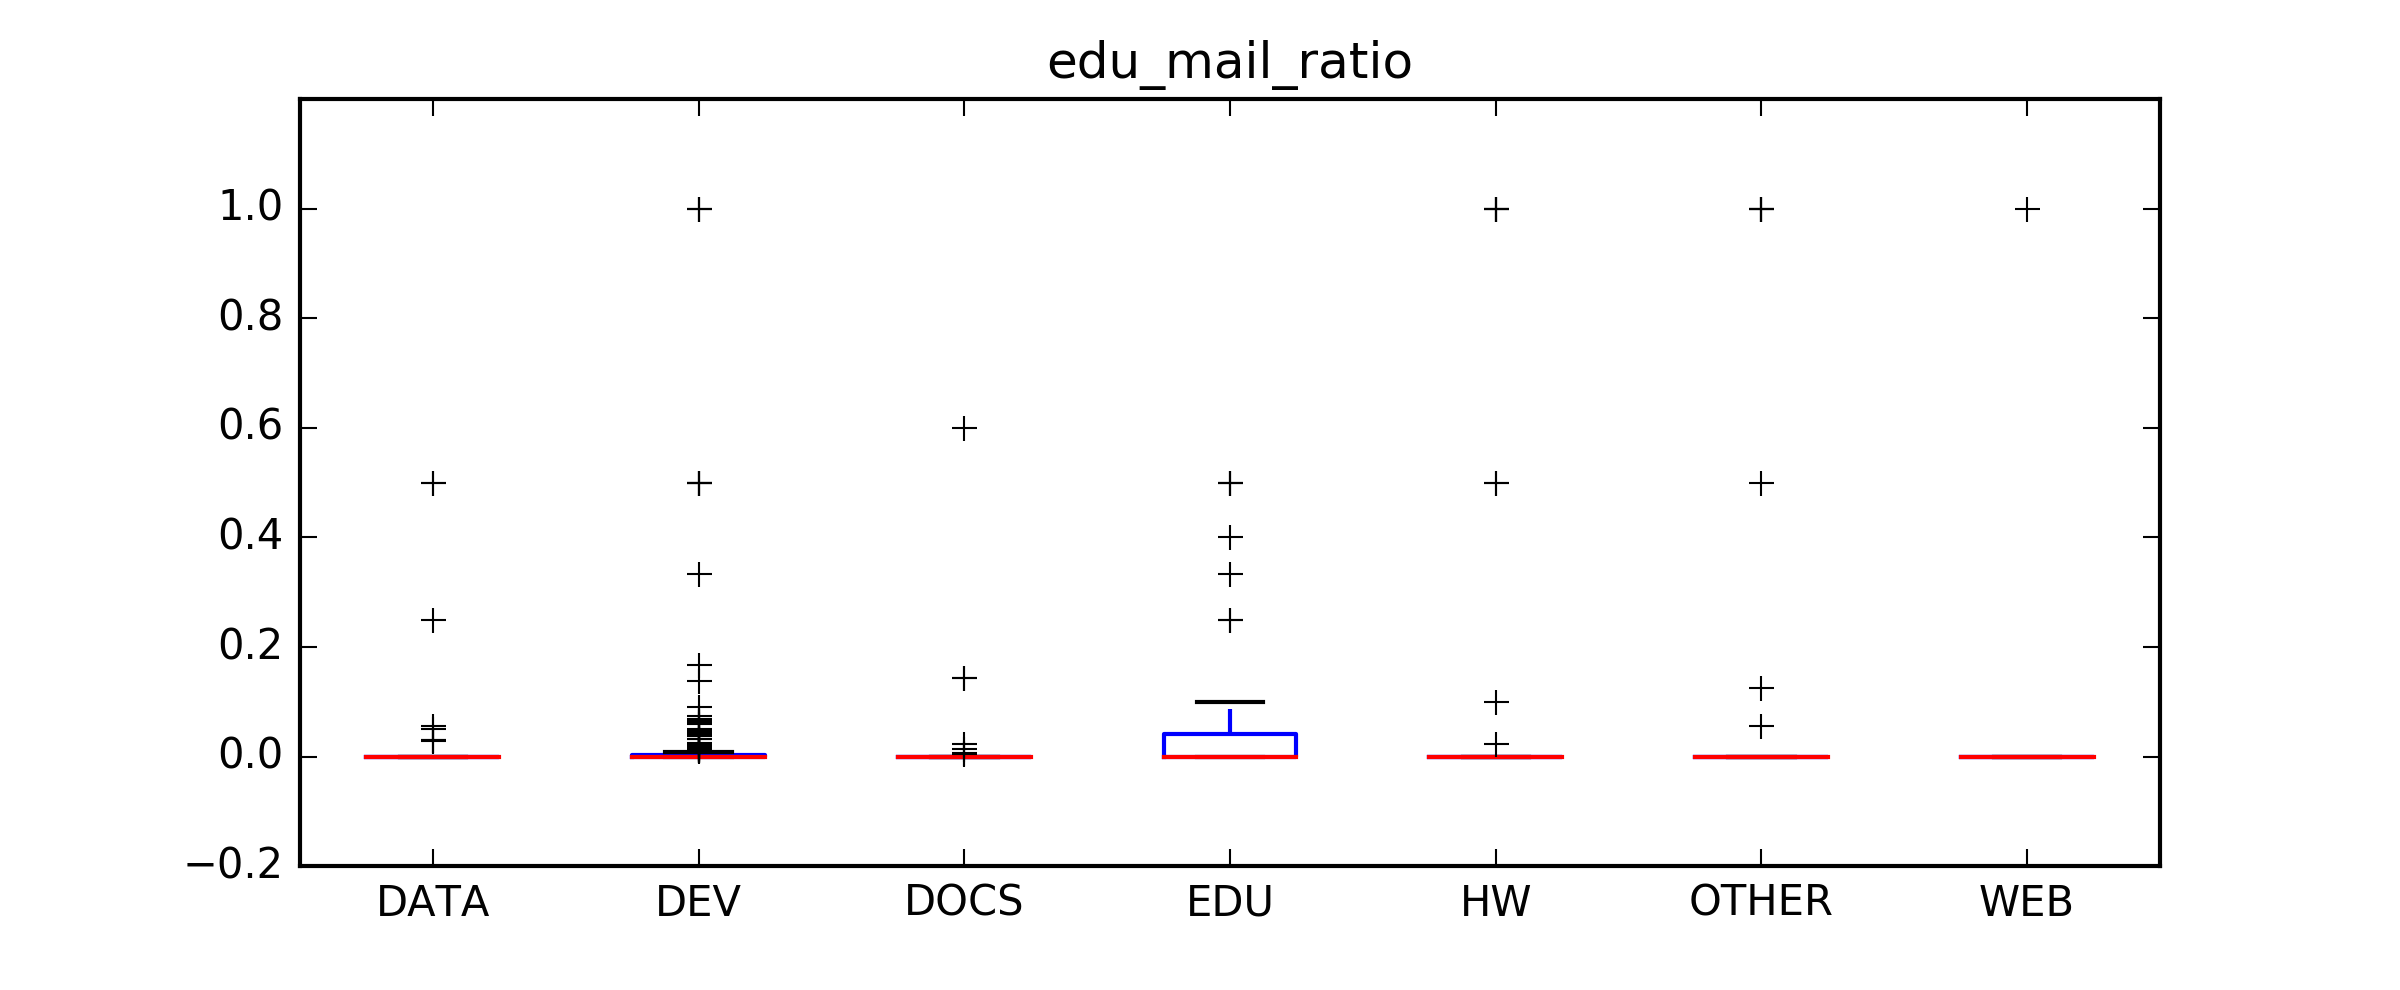
\includegraphics[width=0.75\linewidth]{figures/edu_mail_ratio.png}
				\end{figure}
			\item[File count]
				This is the number files in the repository excluding the .git directory. Additionally we calculate the ratio of specific file types to the total file count. There are metrics for each of the following file types: pdf, html, png, latex, source code and markdown. We identify these file types by the file extension.
				\begin{figure}[h!]
					\centering
					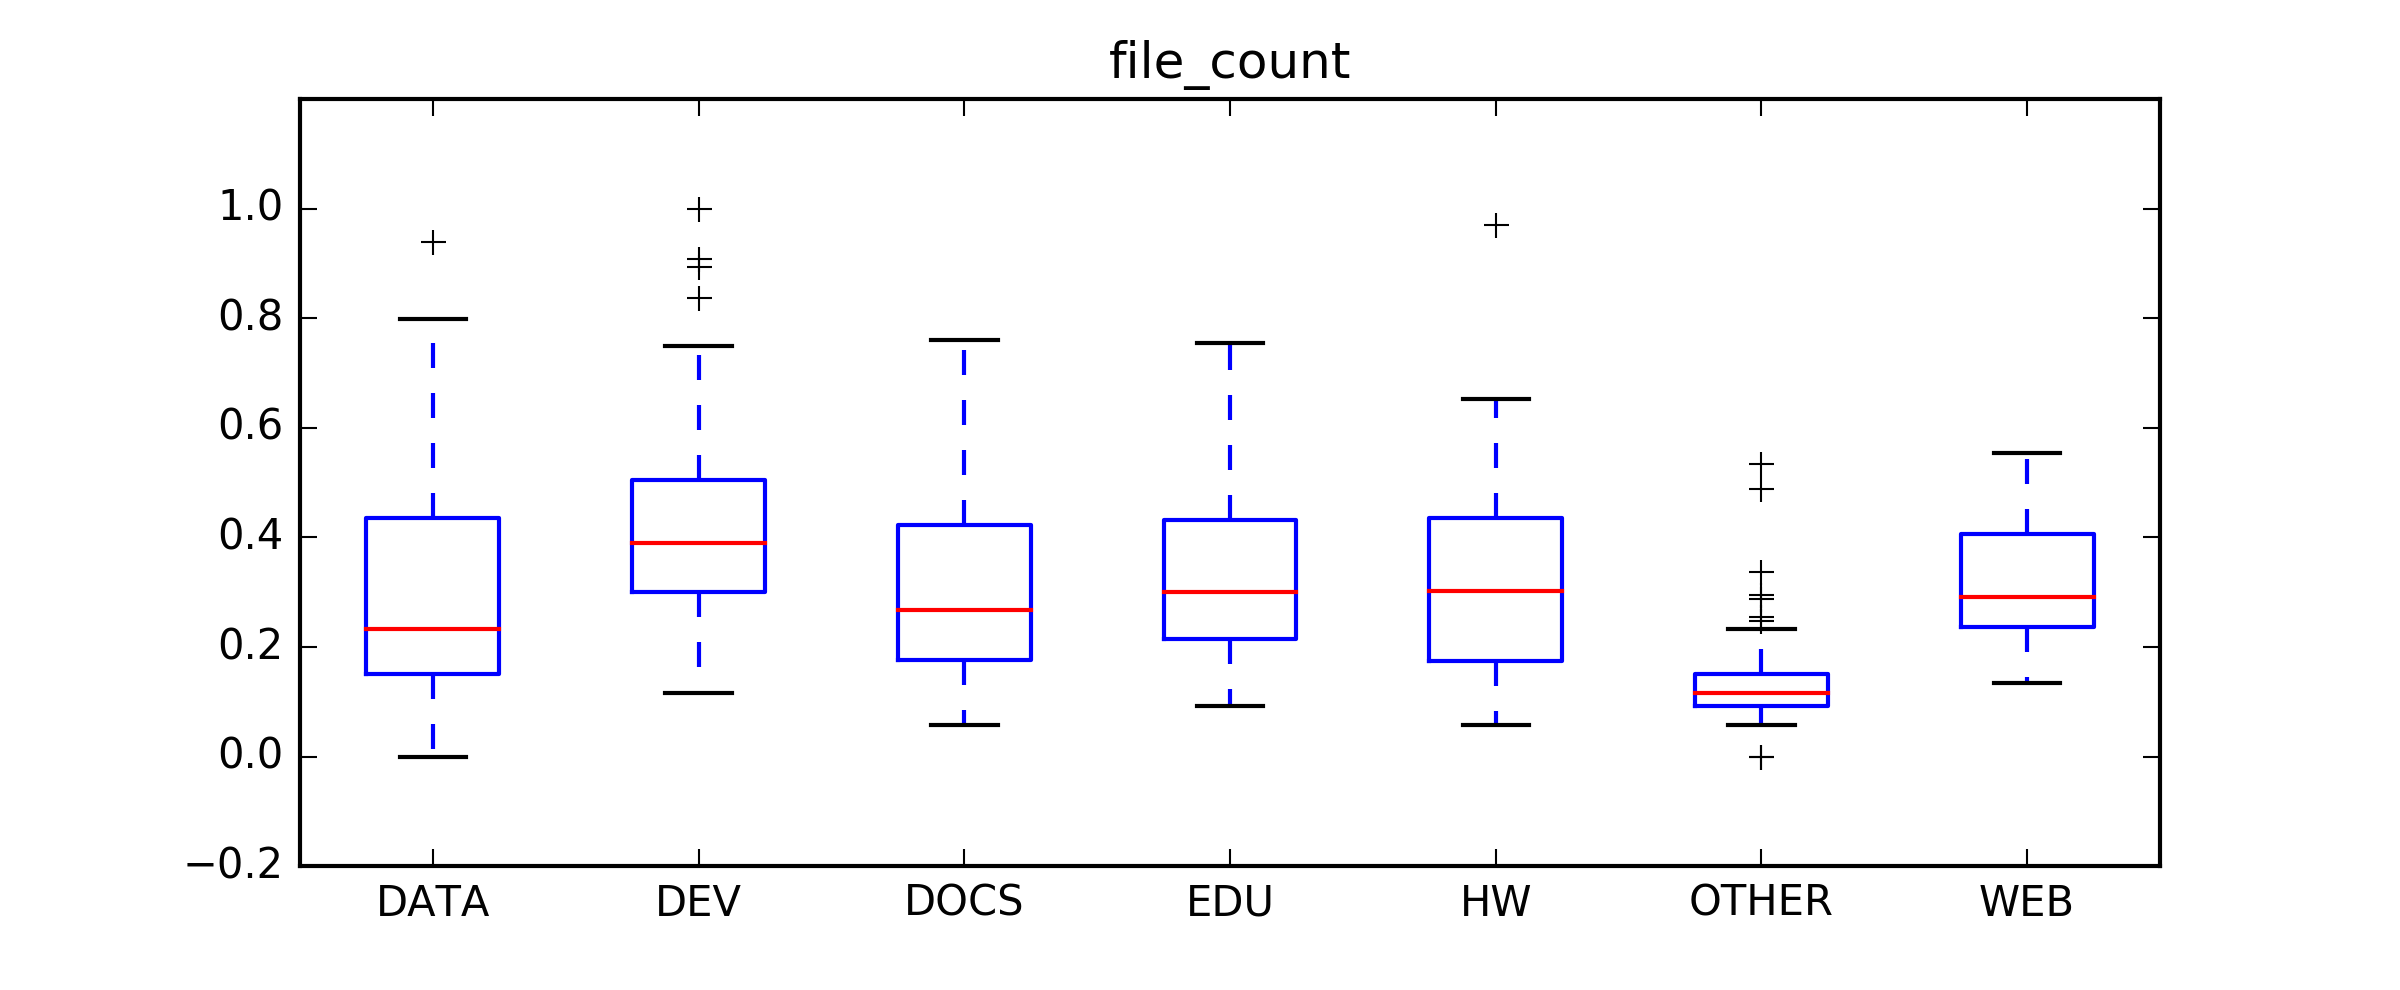
\includegraphics[width=0.75\linewidth]{figures/file_count.png}
				\end{figure}
			\item[File to folder ratio]
				This calculates the ratio between number of files and directories. We expect the DOCS and some DEV (e.g. java programs) to have a low file-folder-ratio.
				\begin{figure}[h!]
					\centering
					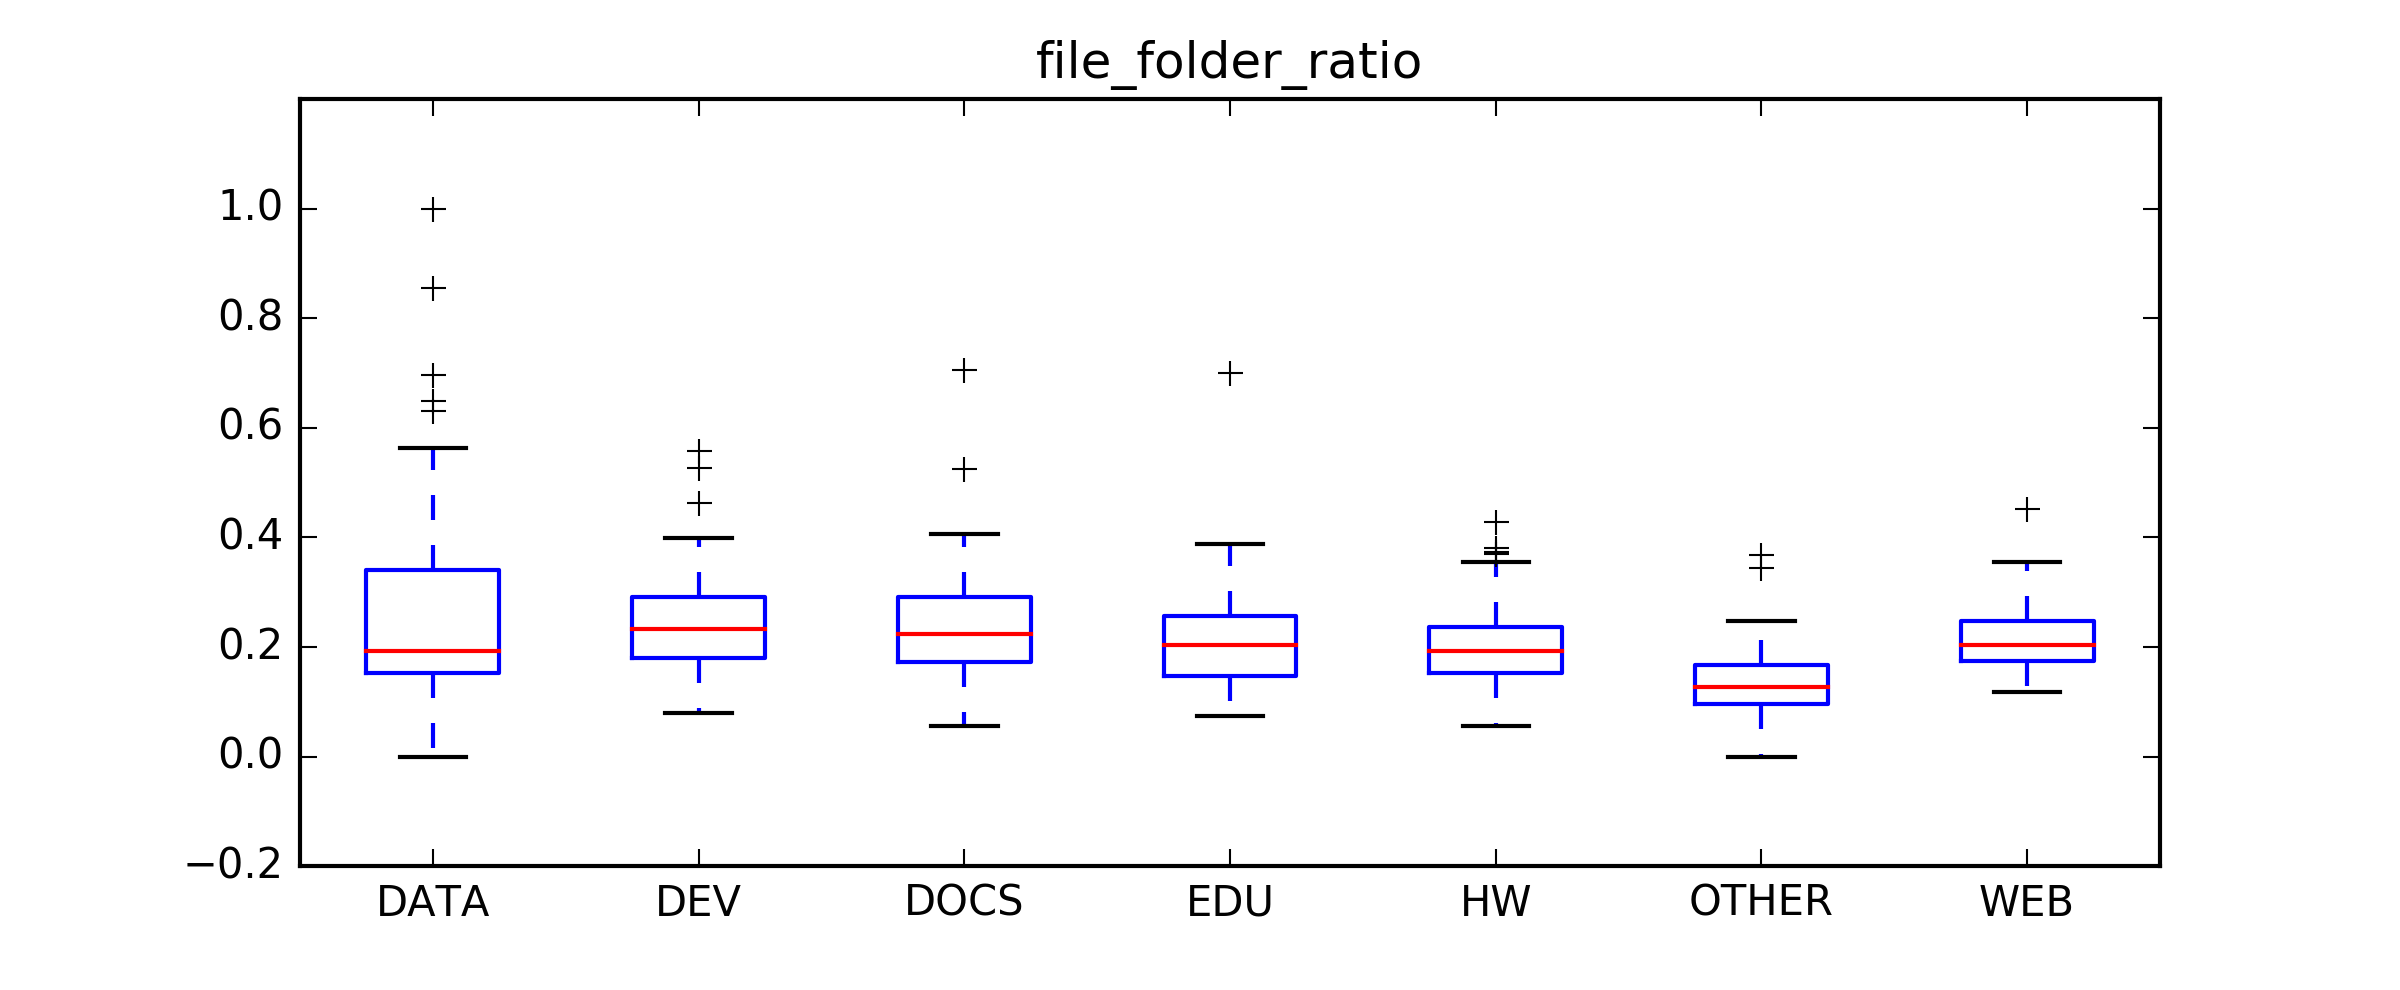
\includegraphics[width=0.75\linewidth]{figures/file_folder_ratio.png}
				\end{figure}
			\item[HTML count]
				This metrics should identify \emph{WEB} repos
				\begin{figure}[h!]
					\centering
					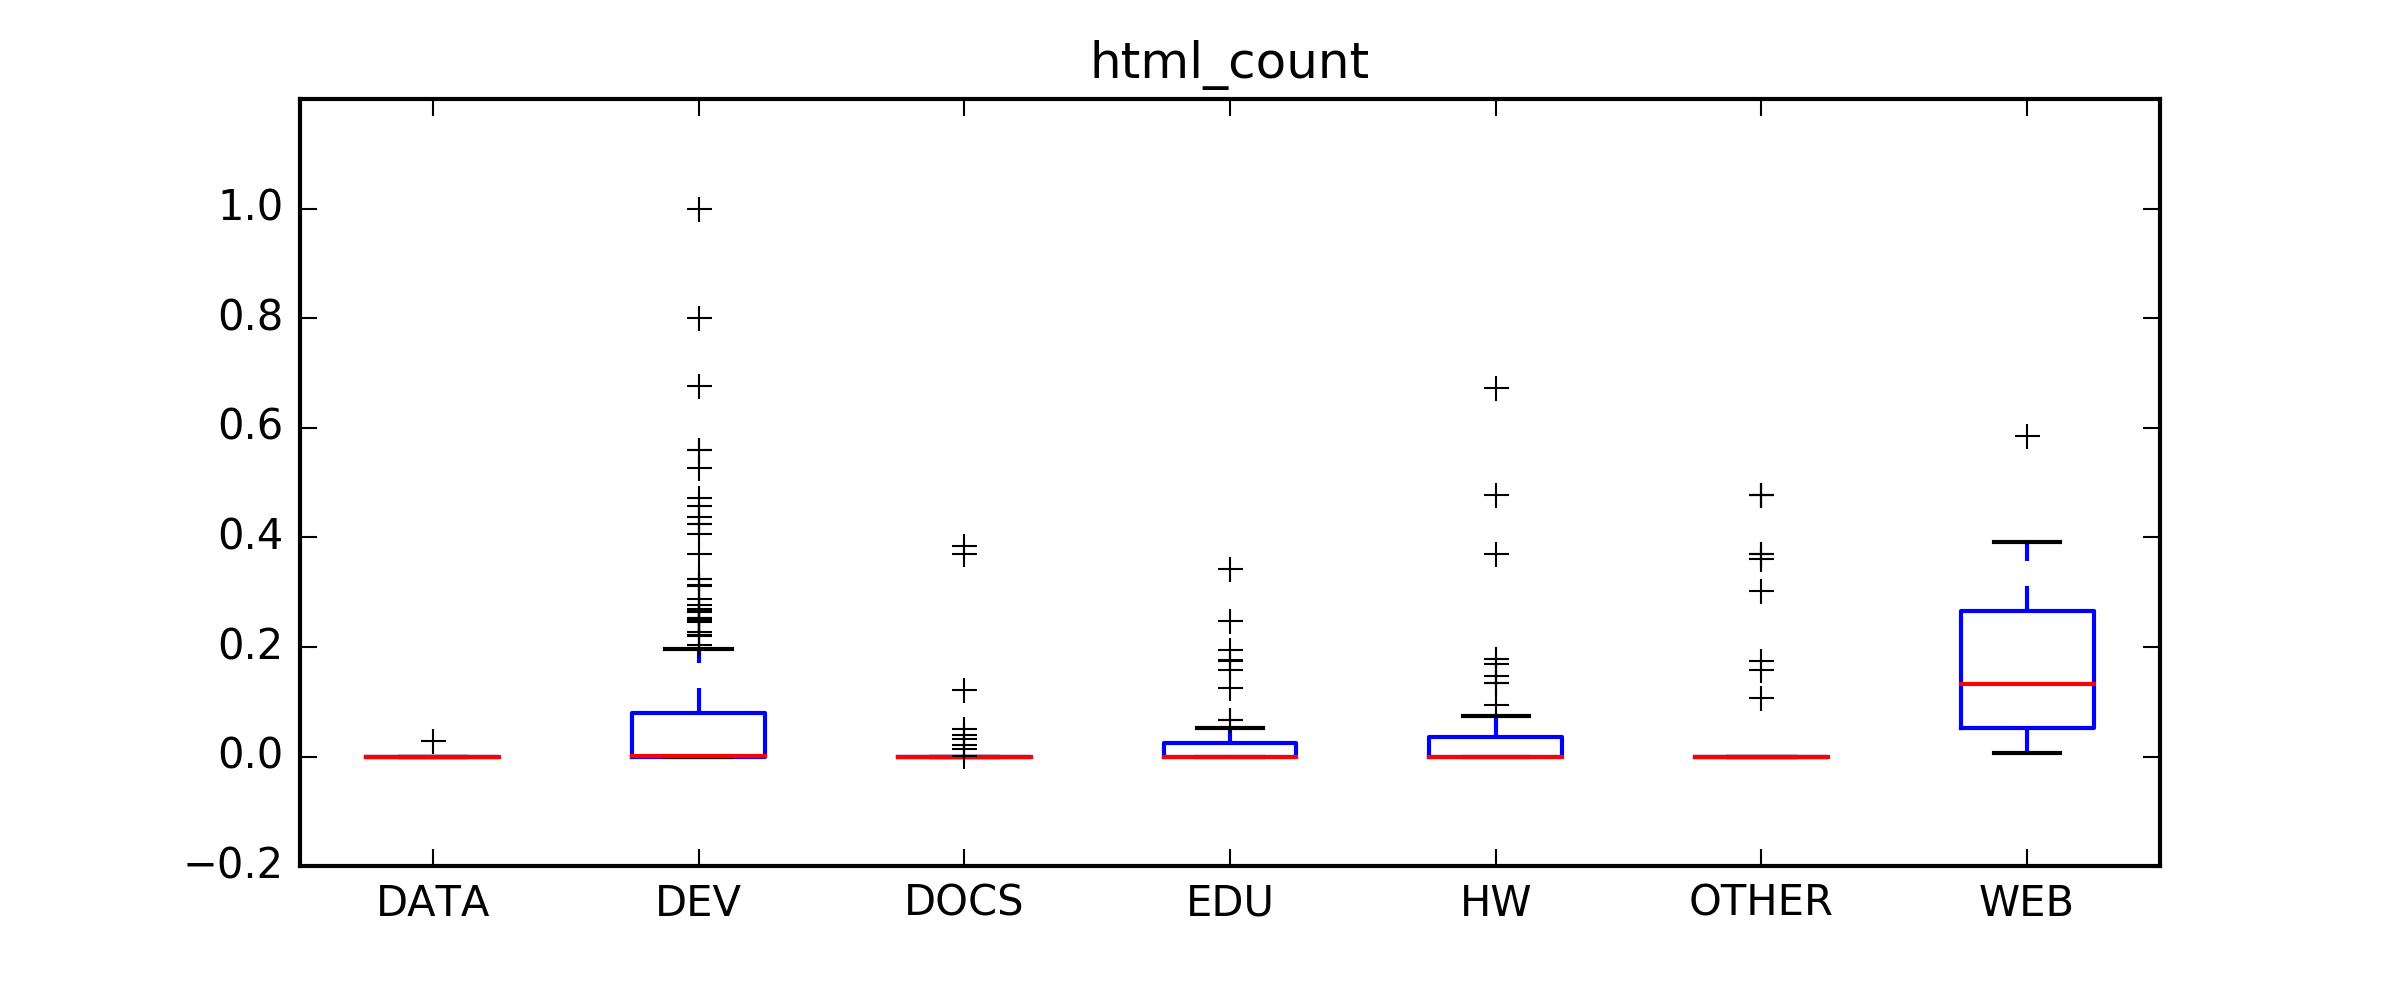
\includegraphics[width=0.75\linewidth]{figures/html_count.png}
				\end{figure}
			\item[HW terminology in commits]
				We search all commit messages for common HW terms and return the number of occurrences. Under common HW terms we understand: 'exercise', 'assignment', 'question', 'task', 'homework', 'student' and 'solution' 
				\begin{figure}[h!]
					\centering
					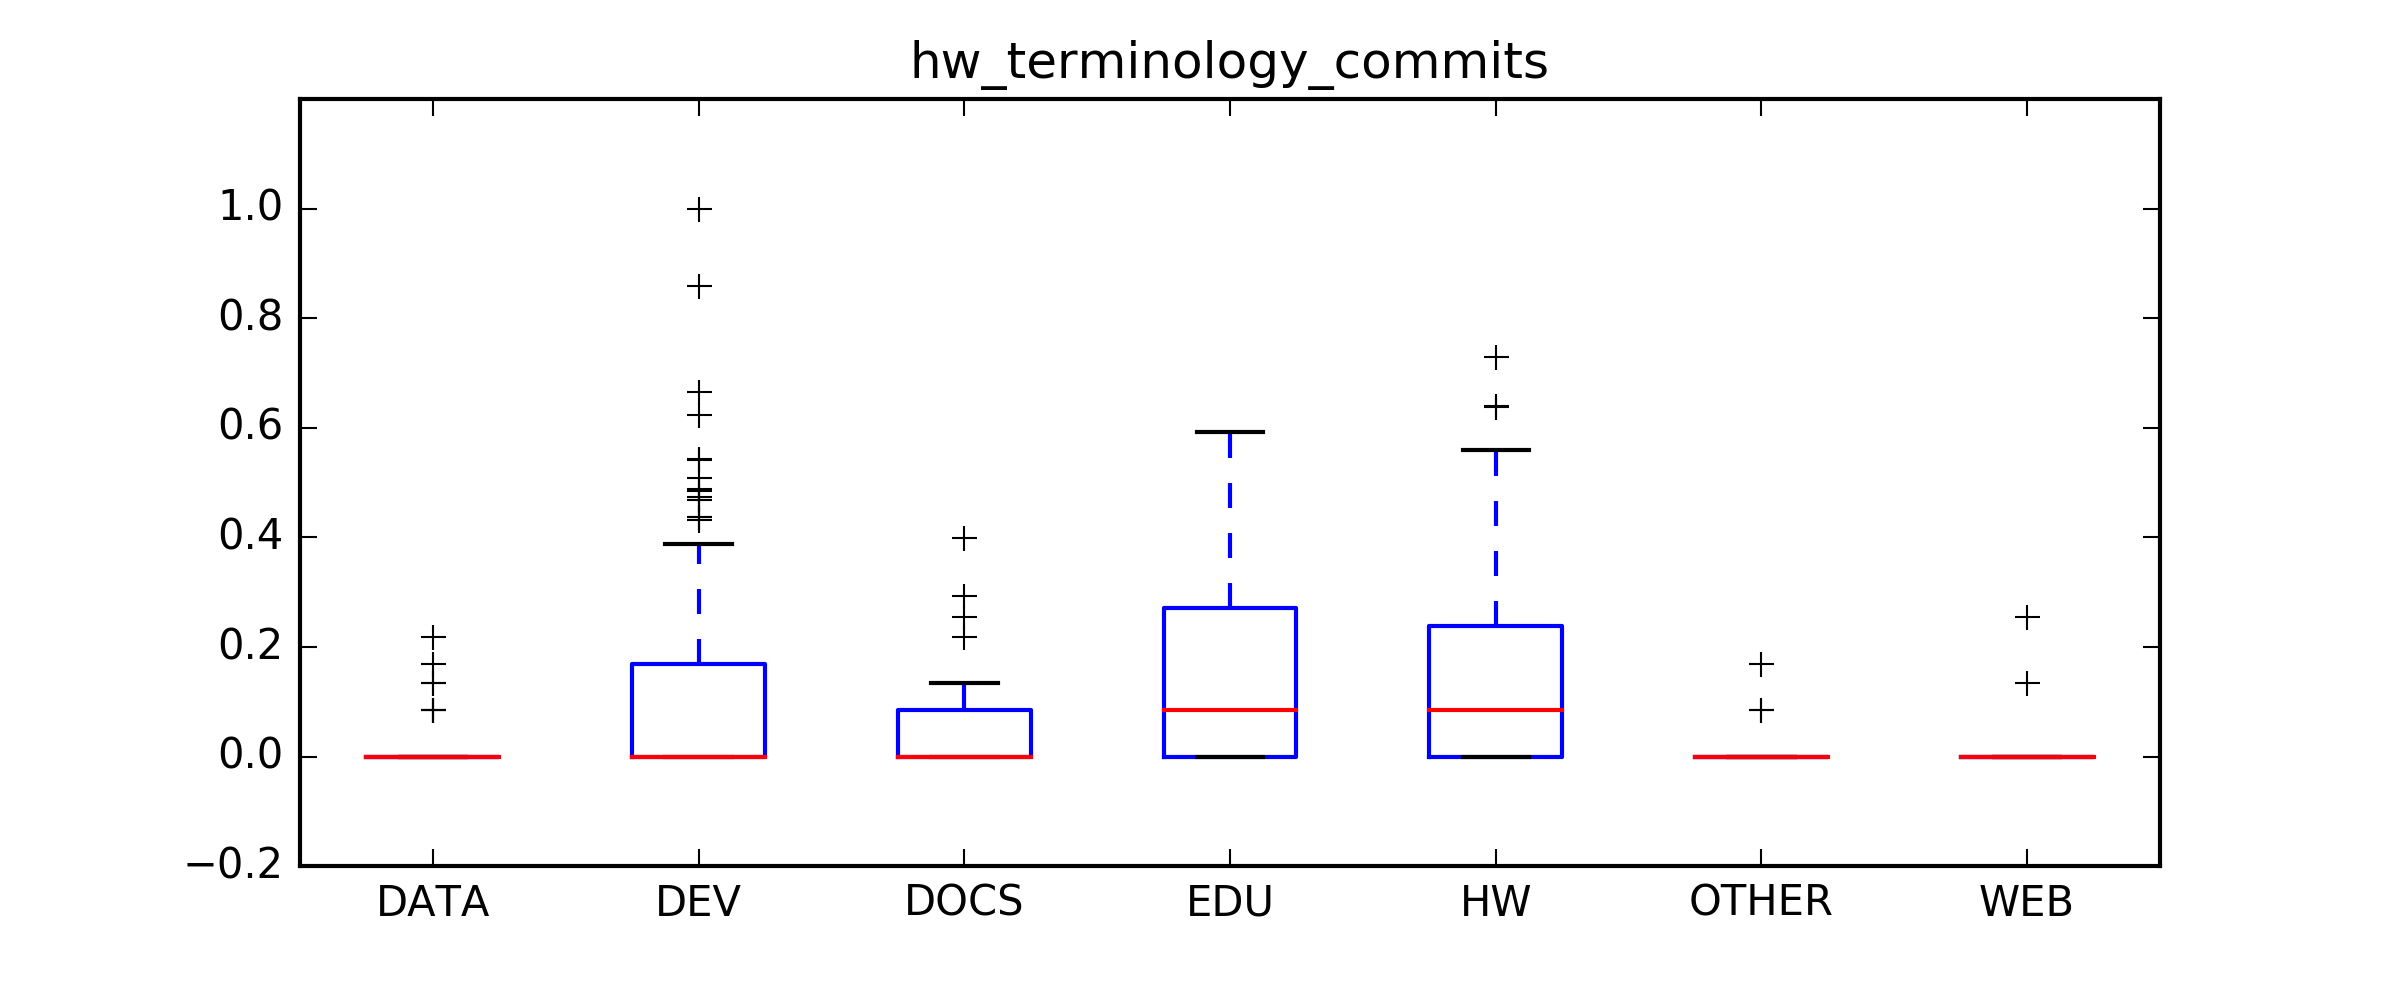
\includegraphics[width=0.75\linewidth]{figures/hw_terminology_commits.png}
				\end{figure}
			\item[HW terminology in filenames or directory names]
				Like HW terminology in commits but we look for the terms in file names.
				\begin{figure}[h!]
					\centering
					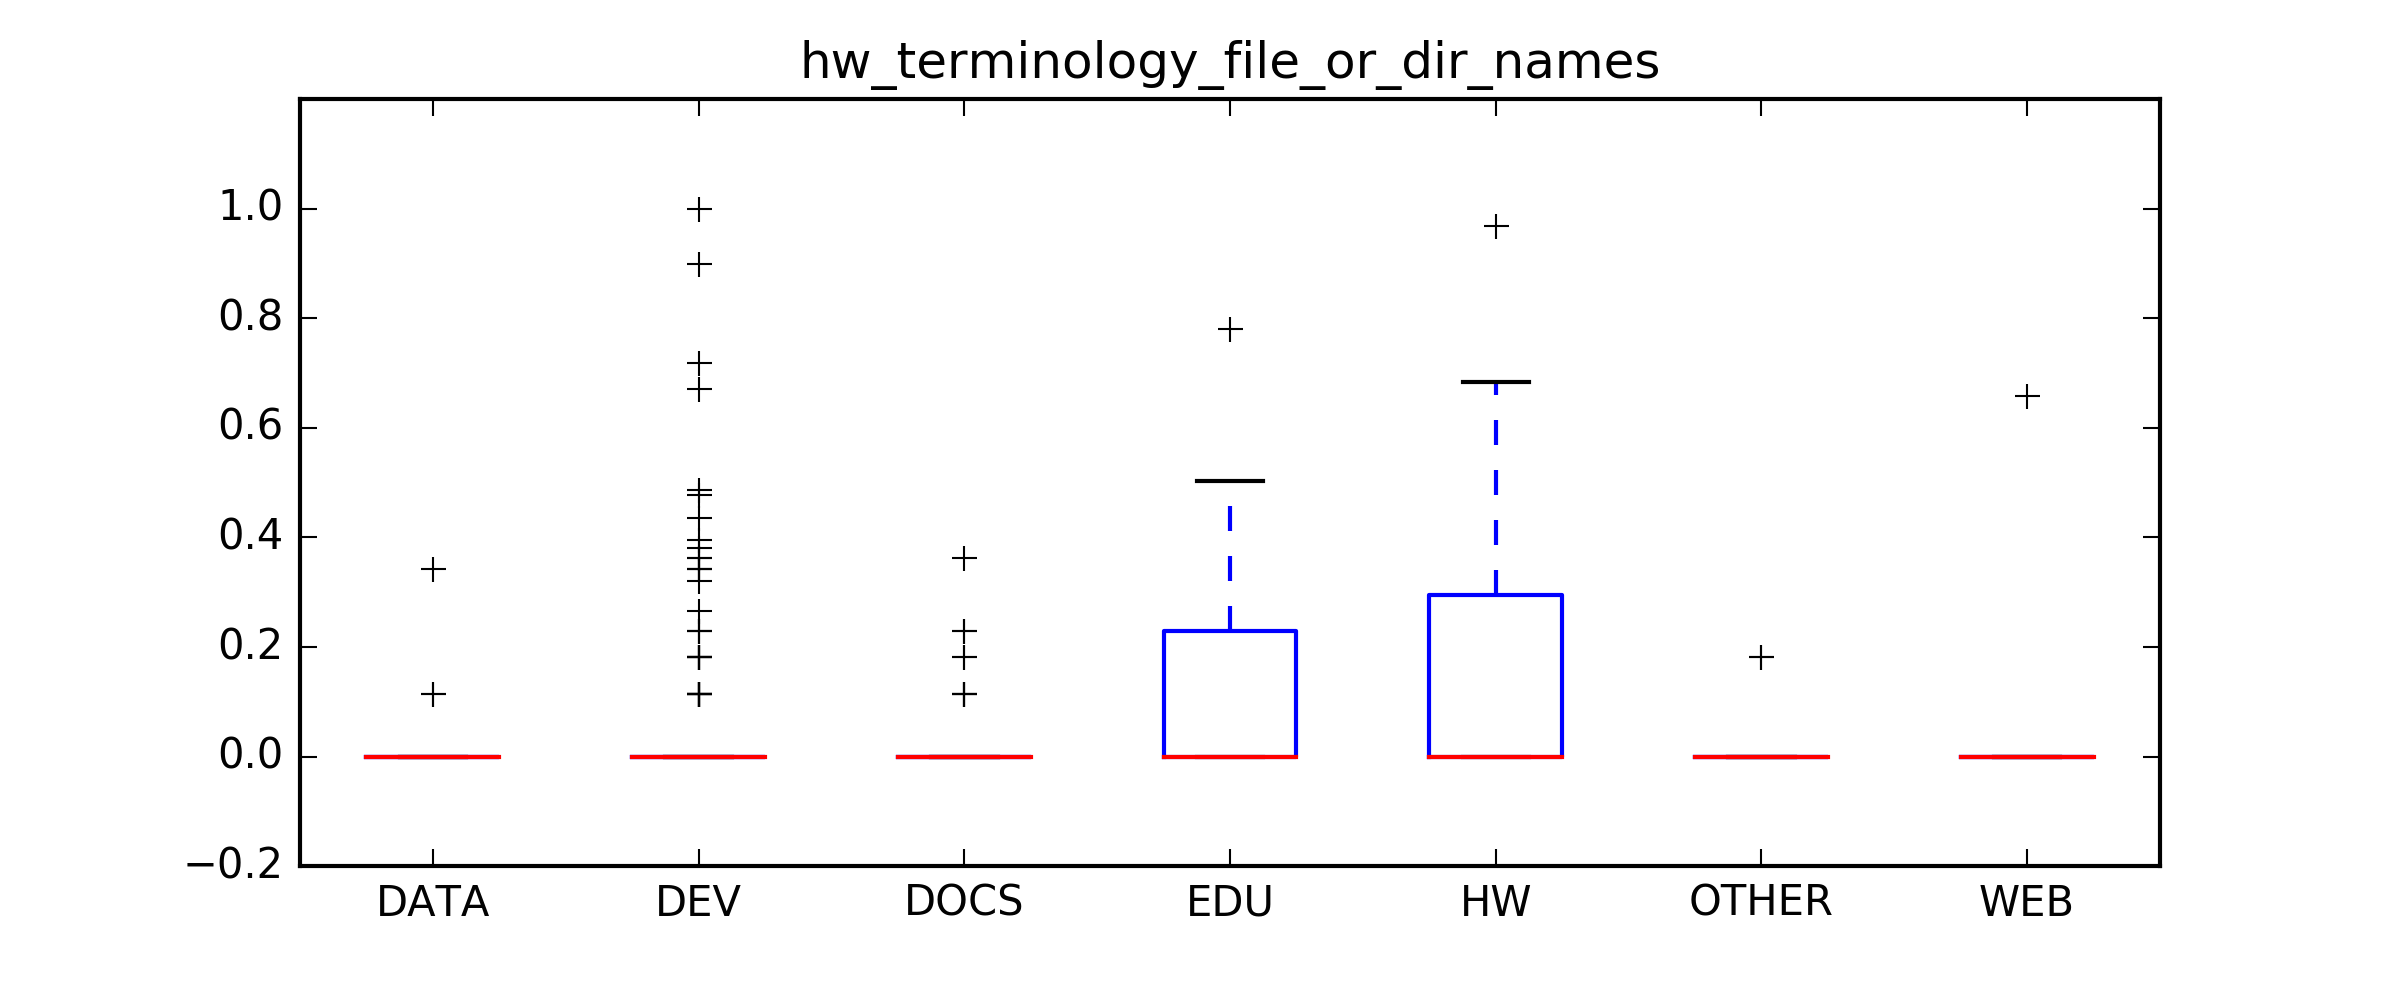
\includegraphics[width=0.75\linewidth]{figures/hw_terminology_file_or_dir_names.png}
				\end{figure}
			\item[md file count]
				Existence of md files indicates \emph{DOCS} and if more than one exists \emph{WEB}
				\begin{figure}[h!]
					\centering
					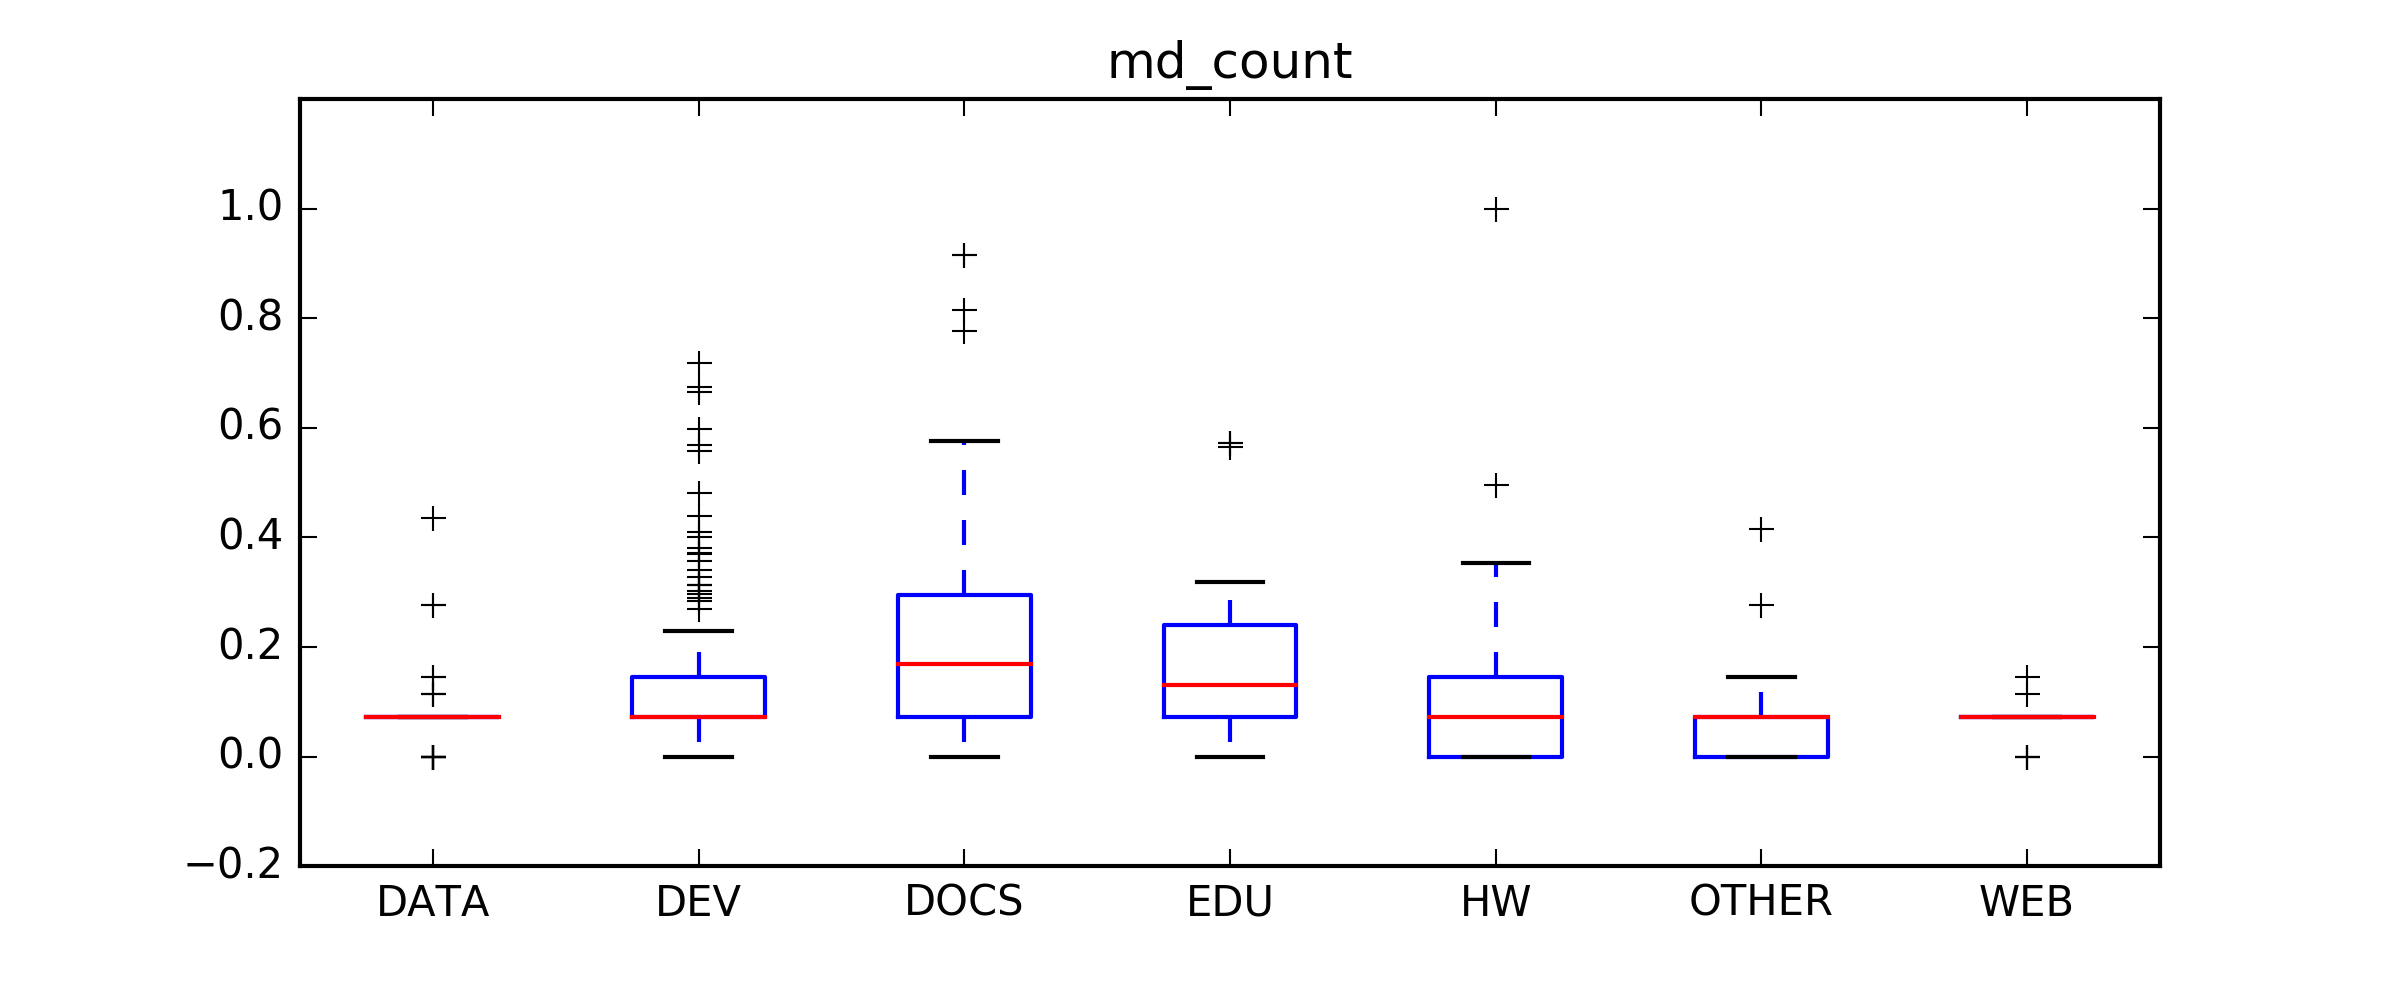
\includegraphics[width=0.75\linewidth]{figures/md_count.png}
				\end{figure}
			\item[pdf count]
				Was supposed to identify \emph{DOCS}, but does not seem to be a strong indicator
				\begin{figure}[h!]
					\centering
					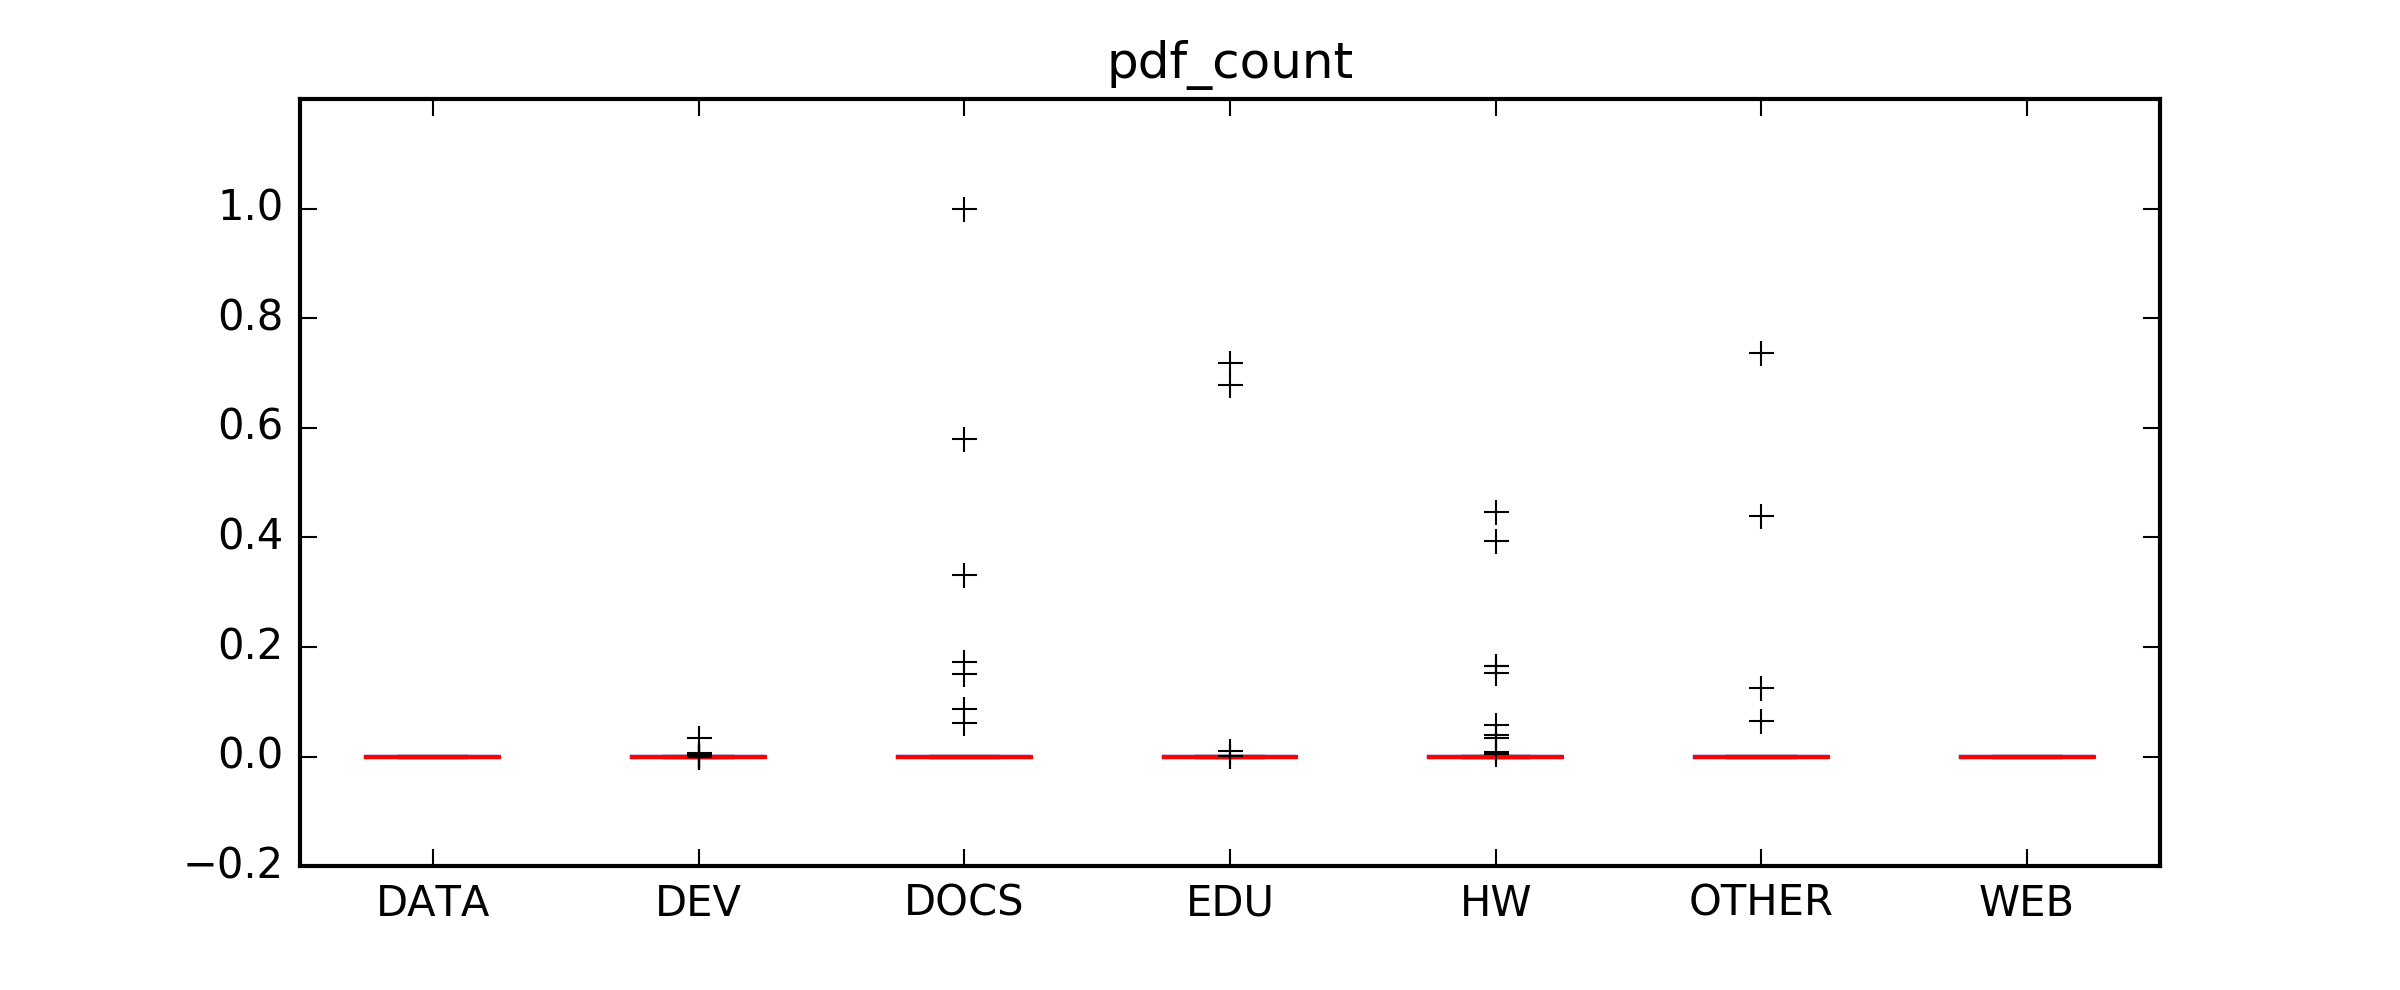
\includegraphics[width=0.75\linewidth]{figures/pdf_count.png}
				\end{figure}
			\item[png count]
				We supposed png to be used for screenshots and info graphics rather than for pictures. This may identify \emph{DOCS} or \emph{EDU}
				\begin{figure}[h!]
					\centering
					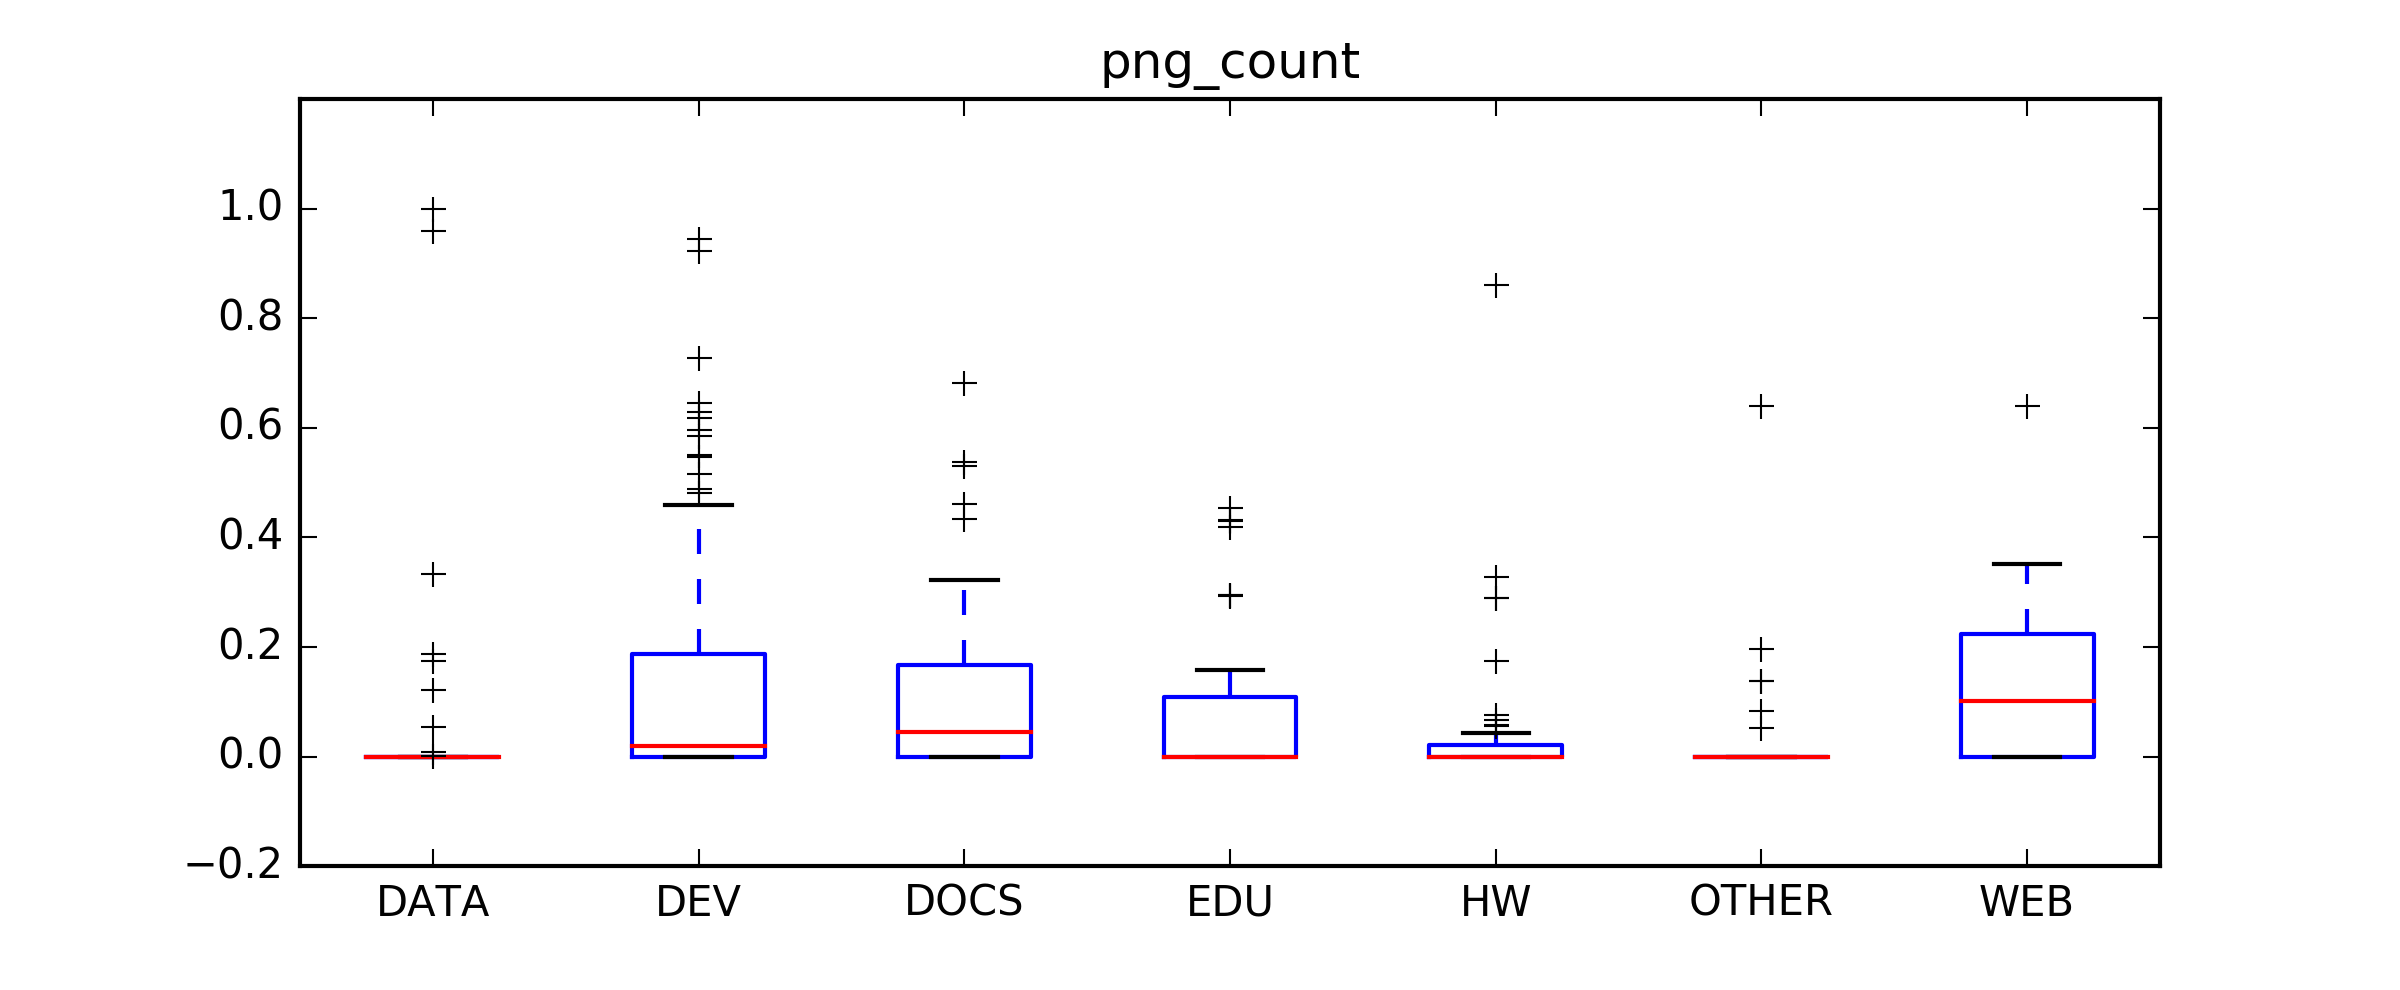
\includegraphics[width=0.75\linewidth]{figures/png_count.png}
				\end{figure}
			\item[source code file ratio]
				Initially thought to identify \emph{DEV} repos
				\begin{figure}[h!]
					\centering
					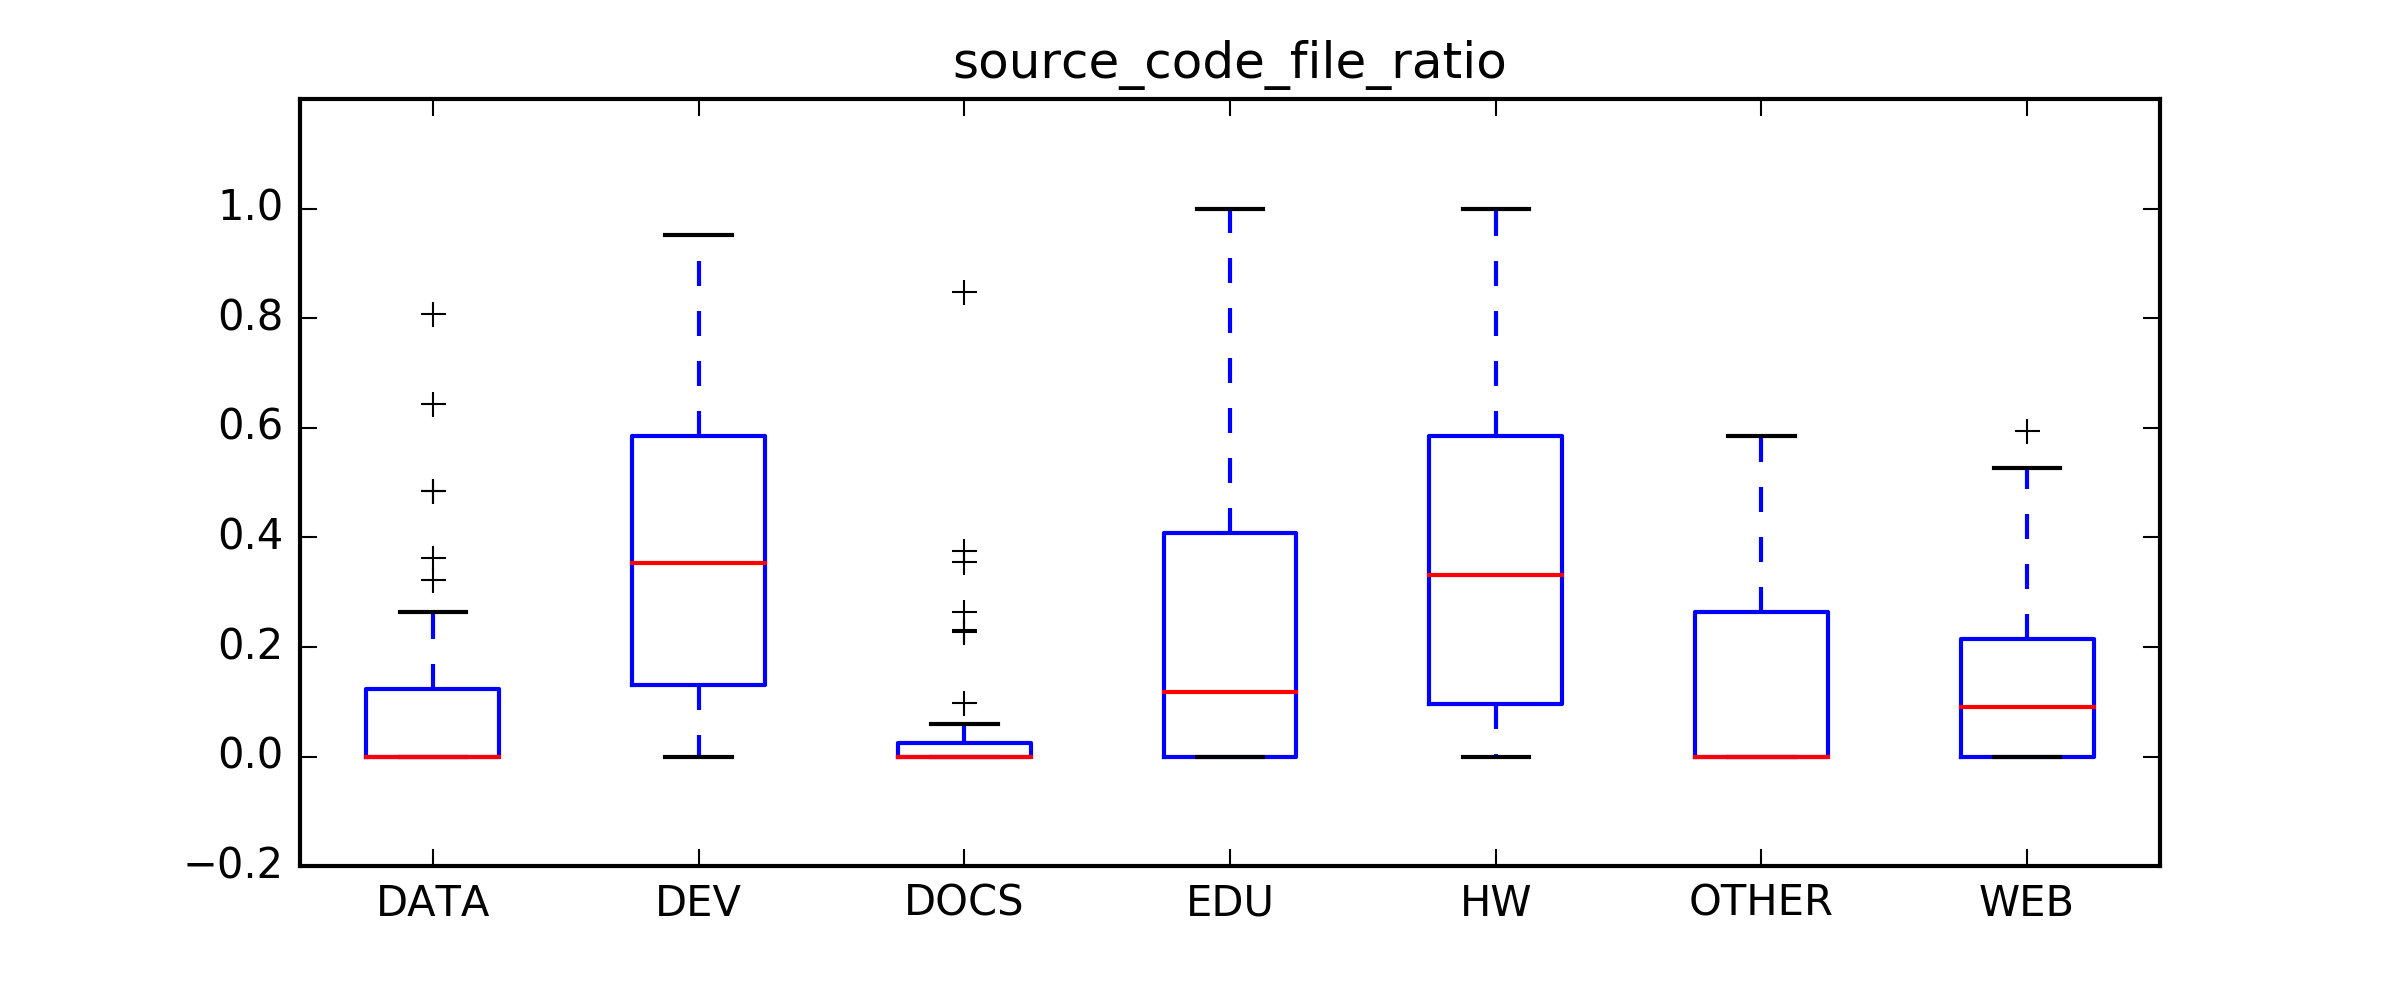
\includegraphics[width=0.75\linewidth]{figures/source_code_file_ratio.png}
				\end{figure}
		\end{description}
		
		% subsubsection cloned_repository (end)

	% subsection metrics_details (end)

% section metrics (end)


\section{Validation}
\label{sec:val}


\section{What we have done}


\section{Program usage}


\end{document}
